\setlength{\tabcolsep}{3pt}
% ===============================================
% 4.1.5.1 ERD tong
% ===============================================
\begin{landscape}
\thispagestyle{landscape}
\Needspace{12\baselineskip}
\subsubsection{Entity Relationship Diagram}

\Needspace{12\baselineskip}
\paragraph{Overall Entity Relationship Diagram}
\label{sec:erd-overall}
\begin{figure}[H]
    \centering
    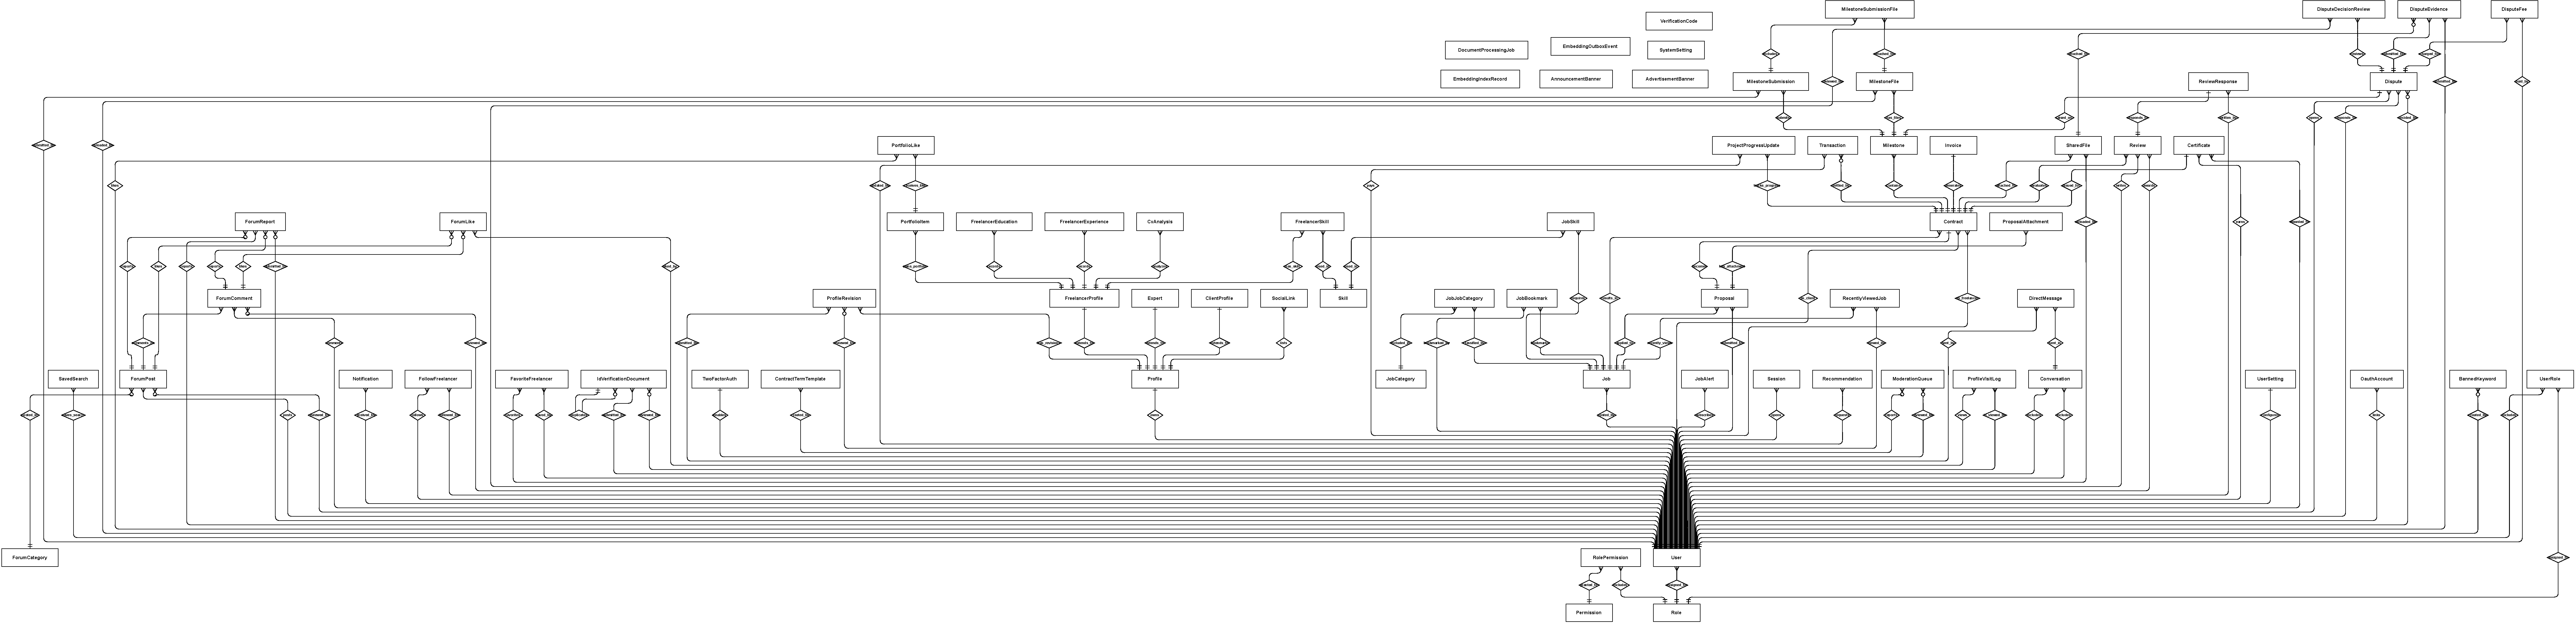
\includegraphics[width=\linewidth]{image/ERD/ERD-ALL.drawio.pdf}
    \caption{Overall Entity Relationship Diagram}
    \label{fig:erd-overall}
\end{figure}
\end{landscape}

% ===============================================
% 4.1.5.2 ERD1
% ===============================================
\Needspace{12\baselineskip}
\paragraph{Authentication \& Sessions}

This ERD describes the Authentication \& Sessions module. It stores account identities, one-time verification codes, device sessions, OAuth links, two-factor authentication settings, and user preferences. User is the root account table and links to Role and Profile. VerificationCode supports registration, email verification, and password reset. Session stores refresh tokens and device information for each login. OauthAccount links Google login to a User. TwoFactorAuth stores the TOTP secret and enabled flag. UserSetting stores theme, language, and notification preferences. These tables support registration, login, logout, password reset, session revocation, Google OAuth, and 2FA.

\Needspace{12\baselineskip}
\paragraph*{a) ERD}
\begin{figure}[H]
    \centering
    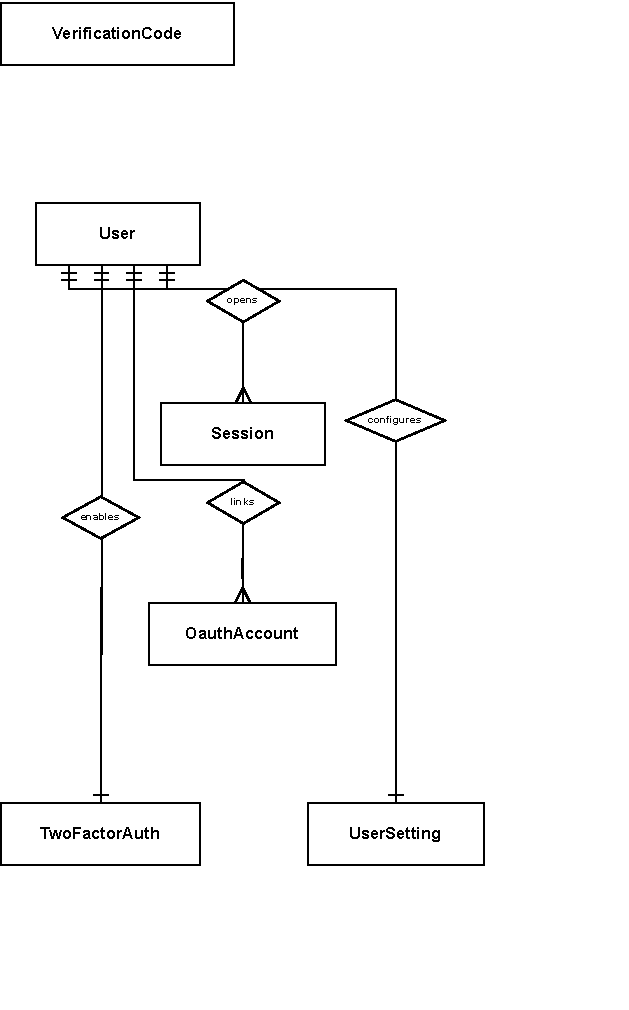
\includegraphics[width=0.78\textwidth]{image/ERD/ERD-ERD1.drawio.pdf}
    \caption{Authentication \& Sessions ERD}
    \label{fig:erd-authentication--sessions}
\end{figure}

\Needspace{8\baselineskip}
\paragraph*{b) Table of entities}\nopagebreak[4]
\begin{center}\nopagebreak[4]
\small\sloppy
\begin{longtable}{|L{2.5cm}|L{9.5cm}|}
\hline
\rowcolor{fptHeader}\textbf{Entity} & \textbf{Fields and descriptions} \\* \hline
\endfirsthead
\hline
\rowcolor{fptHeader}\textbf{Entity} & \textbf{Fields and descriptions} \\* \hline
\endhead
\hline\endfoot
\endlastfoot
\texttt{User} & - id: used to store the unique identifier of the record \\*
& - email: used to store the account email address \\
& - password: used to store the hashed account password \\
& - is\allowbreak Banned: used to store whether the account is banned \\
& - created\allowbreak At: used to store the creation timestamp \\
& - updated\allowbreak At: used to store the last update timestamp \\
& - deleted\allowbreak At: used to store the soft-deletion timestamp \\
& - stripe\allowbreak Customer\allowbreak Id: used to store the stripe customer id text value \\
& - stripe\allowbreak Account\allowbreak Id: used to store the stripe account id text value \\
& - stripe\allowbreak Onboarding\allowbreak Completed: used to store whether Stripe onboarding is completed \\
& - role\allowbreak Id: used to store the foreign key reference to the primary role \\ \hline
\texttt{Verification\allowbreak Code} & - id: used to store the unique identifier of the record \\*
& - email: used to store the account email address \\
& - code: used to store the one-time verification code \\
& - type: used to store the type value from the VerificationCodeType enumeration \\
& - attempts: used to store the verification attempt count \\
& - expires\allowbreak At: used to store the expiration timestamp \\
& - created\allowbreak At: used to store the creation timestamp \\ \hline
\texttt{Session} & - id: used to store the unique identifier of the record \\*
& - user\allowbreak Id: used to store the foreign key reference to the user \\
& - refresh\allowbreak Token: used to store the refresh token \\
& - device\allowbreak Info: used to store the device information text \\
& - ip\allowbreak Address: used to store the IP address \\
& - expires\allowbreak At: used to store the expiration timestamp \\
& - created\allowbreak At: used to store the creation timestamp \\ \hline
\texttt{Oauth\allowbreak Account} & - id: used to store the unique identifier of the record \\*
& - user\allowbreak Id: used to store the foreign key reference to the user \\
& - provider: used to store the provider value from the OauthProvider enumeration \\
& - provider\allowbreak User\allowbreak Id: used to store the external provider user identifier \\
& - created\allowbreak At: used to store the creation timestamp \\ \hline
\texttt{Two\allowbreak Factor\allowbreak Auth} & - id: used to store the unique identifier of the record \\*
& - user\allowbreak Id: used to store the foreign key reference to the user \\
& - secret: used to store the TOTP secret value \\
& - enabled: used to store whether two-factor authentication is enabled \\
& - created\allowbreak At: used to store the creation timestamp \\ \hline
\texttt{User\allowbreak Setting} & - id: used to store the unique identifier of the record \\*
& - user\allowbreak Id: used to store the foreign key reference to the user \\
& - theme: used to store the theme text value \\
& - language: used to store the language text value \\
& - notification\allowbreak Prefs: used to store the notification preferences data in JSON format \\ \hline
\end{longtable}
\end{center}

% ===============================================
% 4.1.5.3 ERD2
% ===============================================
\Needspace{12\baselineskip}
\paragraph{Role-Based Access Control}

This ERD describes the Role-Based Access Control module. It stores roles, permissions, role-permission assignments, and user-role assignments. Role defines a named role; Permission defines a route-level permission; RolePermission links permissions to roles; UserRole links users to roles. These tables support RBAC guards, permission checks, and role switching without redeployment.

\Needspace{12\baselineskip}
\paragraph*{a) ERD}
\begin{figure}[H]
    \centering
    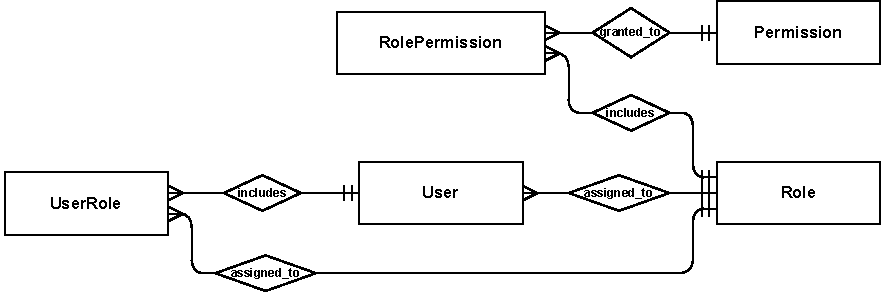
\includegraphics[width=0.78\textwidth]{image/ERD/ERD-ERD2.drawio.pdf}
    \caption{Role-Based Access Control ERD}
    \label{fig:erd-role-based-access-control}
\end{figure}

\Needspace{8\baselineskip}
\paragraph*{b) Table of entities}\nopagebreak[4]
\begin{center}\nopagebreak[4]
\small\sloppy
\begin{longtable}{|L{2.5cm}|L{9.5cm}|}
\hline
\rowcolor{fptHeader}\textbf{Entity} & \textbf{Fields and descriptions} \\* \hline
\endfirsthead
\hline
\rowcolor{fptHeader}\textbf{Entity} & \textbf{Fields and descriptions} \\* \hline
\endhead
\hline\endfoot
\endlastfoot
\texttt{User} & - id: used to store the unique identifier of the record \\*
& - email: used to store the account email address \\
& - password: used to store the hashed account password \\
& - is\allowbreak Banned: used to store whether the account is banned \\
& - created\allowbreak At: used to store the creation timestamp \\
& - updated\allowbreak At: used to store the last update timestamp \\
& - deleted\allowbreak At: used to store the soft-deletion timestamp \\
& - stripe\allowbreak Customer\allowbreak Id: used to store the stripe customer id text value \\
& - stripe\allowbreak Account\allowbreak Id: used to store the stripe account id text value \\
& - stripe\allowbreak Onboarding\allowbreak Completed: used to store whether Stripe onboarding is completed \\
& - role\allowbreak Id: used to store the foreign key reference to the primary role \\ \hline
\texttt{Role} & - id: used to store the unique identifier of the record \\*
& - name: used to store the name value \\
& - description: used to store the description text \\
& - created\allowbreak At: used to store the creation timestamp \\
& - deleted\allowbreak At: used to store the soft-deletion timestamp \\ \hline
\texttt{User\allowbreak Role} & - user\allowbreak Id: used to store the foreign key reference to the user \\*
& - role\allowbreak Id: used to store the foreign key reference to the primary role \\
& - assigned\allowbreak At: used to store the assigned at timestamp \\ \hline
\texttt{Permission} & - id: used to store the unique identifier of the record \\*
& - name: used to store the name value \\
& - path: used to store the route path \\
& - method: used to store the HTTP method value from the HttpMethod enumeration \\
& - module: used to store the module name \\
& - created\allowbreak By\allowbreak Id: used to store the created by id integer value \\
& - updated\allowbreak By\allowbreak Id: used to store the updated by id integer value \\
& - deleted\allowbreak By\allowbreak Id: used to store the deleted by id integer value \\
& - deleted\allowbreak At: used to store the soft-deletion timestamp \\
& - created\allowbreak At: used to store the creation timestamp \\
& - updated\allowbreak At: used to store the last update timestamp \\ \hline
\texttt{Role\allowbreak Permission} & - role\allowbreak Id: used to store the foreign key reference to the primary role \\*
& - permission\allowbreak Id: used to store the foreign key reference to the permission \\ \hline
\end{longtable}
\end{center}

% ===============================================
% 4.1.5.4 ERD3
% ===============================================
\Needspace{12\baselineskip}
\paragraph{Profile Core}

This ERD describes the Profile Core module. It stores base profiles and role-specific profile extensions. Profile contains common display information; FreelancerProfile stores professional data; ClientProfile stores company data; Expert publishes expert directory entries; FreelancerSkill links freelancers to skills with proficiency. These tables support profile viewing/editing, freelancer/client/expert profiles, skills, and profile completion.

\Needspace{12\baselineskip}
\paragraph*{a) ERD}
\begin{figure}[H]
    \centering
    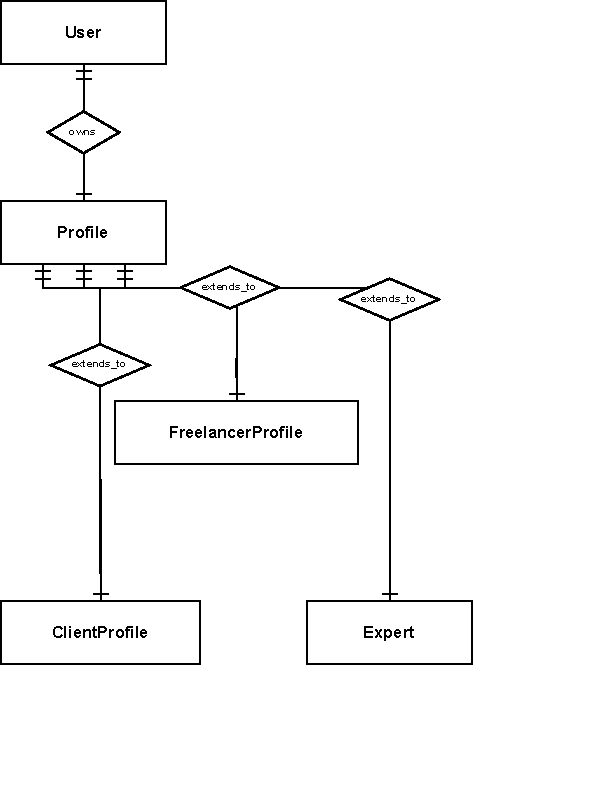
\includegraphics[width=0.78\textwidth]{image/ERD/ERD-ERD3.drawio.pdf}
    \caption{Profile Core ERD}
    \label{fig:erd-profile-core}
\end{figure}

\Needspace{8\baselineskip}
\paragraph*{b) Table of entities}\nopagebreak[4]
\begin{center}\nopagebreak[4]
\small\sloppy
\begin{longtable}{|L{2.5cm}|L{9.5cm}|}
\hline
\rowcolor{fptHeader}\textbf{Entity} & \textbf{Fields and descriptions} \\* \hline
\endfirsthead
\hline
\rowcolor{fptHeader}\textbf{Entity} & \textbf{Fields and descriptions} \\* \hline
\endhead
\hline\endfoot
\endlastfoot
\texttt{User} & - id: used to store the unique identifier of the record \\*
& - email: used to store the account email address \\
& - password: used to store the hashed account password \\
& - is\allowbreak Banned: used to store whether the account is banned \\
& - created\allowbreak At: used to store the creation timestamp \\
& - updated\allowbreak At: used to store the last update timestamp \\
& - deleted\allowbreak At: used to store the soft-deletion timestamp \\
& - stripe\allowbreak Customer\allowbreak Id: used to store the stripe customer id text value \\
& - stripe\allowbreak Account\allowbreak Id: used to store the stripe account id text value \\
& - stripe\allowbreak Onboarding\allowbreak Completed: used to store whether Stripe onboarding is completed \\
& - role\allowbreak Id: used to store the foreign key reference to the primary role \\ \hline
\texttt{Profile} & - id: used to store the unique identifier of the record \\*
& - user\allowbreak Id: used to store the foreign key reference to the user \\
& - display\allowbreak Name: used to store the display name text value \\
& - avatar\allowbreak Url: used to store the avatar file URL \\
& - cover\allowbreak Url: used to store the cover image URL \\
& - bio: used to store the bio text value \\
& - online\allowbreak Status: used to store the online status flag \\
& - availability\allowbreak Status: used to store the availability status value from the AvailabilityStatus enumeration \\
& - profile\allowbreak Completion\allowbreak Percent: used to store the profile completion percentage \\
& - wallet\allowbreak Address: used to store the wallet address \\
& - created\allowbreak At: used to store the creation timestamp \\
& - updated\allowbreak At: used to store the last update timestamp \\ \hline
\texttt{Freelancer\allowbreak Profile} & - id: used to store the unique identifier of the record \\*
& - profile\allowbreak Id: used to store the foreign key reference to the profile \\
& - title: used to store the title text \\
& - education: used to store the list of education \\
& - certifications: used to store the list of certifications \\
& - languages: used to store the list of languages \\
& - cv\allowbreak Url: used to store the uploaded CV file URL \\
& - cv\allowbreak File\allowbreak Name: used to store the cv file name text value \\
& - cv\allowbreak Public\allowbreak Id: used to store the cv public id text value \\
& - cv\allowbreak Uploaded\allowbreak At: used to store the cv uploaded at timestamp \\
& - experience: used to store the list of experience \\
& - id\allowbreak Verified: used to store whether the identity is verified \\
& - created\allowbreak At: used to store the creation timestamp \\
& - updated\allowbreak At: used to store the last update timestamp \\ \hline
\texttt{Client\allowbreak Profile} & - id: used to store the unique identifier of the record \\*
& - profile\allowbreak Id: used to store the foreign key reference to the profile \\
& - company\allowbreak Name: used to store the company name text value \\
& - company\allowbreak Description: used to store the company description text value \\
& - website: used to store the website text value \\
& - created\allowbreak At: used to store the creation timestamp \\
& - updated\allowbreak At: used to store the last update timestamp \\ \hline
\texttt{Expert} & - id: used to store the unique identifier of the record \\*
& - profile\allowbreak Id: used to store the foreign key reference to the profile \\
& - title: used to store the title text \\
& - expertise: used to store the list of expertise \\
& - years\allowbreak Of\allowbreak Experience: used to store the years of experience \\
& - education: used to store the list of education \\
& - certifications: used to store the list of certifications \\
& - website: used to store the website text value \\
& - is\allowbreak Active: used to store whether the record is active \\
& - created\allowbreak At: used to store the creation timestamp \\
& - updated\allowbreak At: used to store the last update timestamp \\ \hline
\end{longtable}
\end{center}

% ===============================================
% 4.1.5.5 ERD4
% ===============================================
\Needspace{12\baselineskip}
\paragraph{Profile History \& Social Links}

This ERD describes the Profile History \& Social Links module. It stores profile revisions, portfolio items, CV analysis, experience, education, document processing jobs, embedding records, recommendations, feedback, embedding outbox events, social links, identity documents, and profile visit logs. These tables support profile revision review, portfolio, CV processing, recommendations, social links, identity verification, and profile visit tracking.

\Needspace{12\baselineskip}
\paragraph*{a) ERD}
\begin{figure}[H]
    \centering
    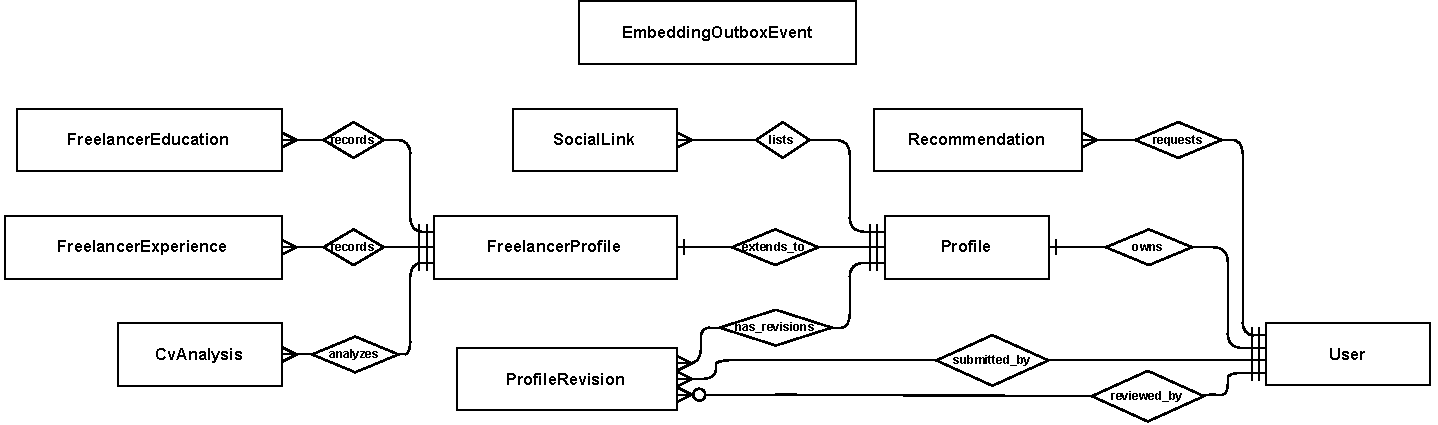
\includegraphics[width=0.78\textwidth]{image/ERD/ERD-ERD4.drawio.pdf}
    \caption{Profile History \& Social Links ERD}
    \label{fig:erd-profile-history--social-links}
\end{figure}

\Needspace{8\baselineskip}
\paragraph*{b) Table of entities}\nopagebreak[4]
\begin{center}\nopagebreak[4]
\small\sloppy
\begin{longtable}{|L{2.5cm}|L{9.5cm}|}
\hline
\rowcolor{fptHeader}\textbf{Entity} & \textbf{Fields and descriptions} \\* \hline
\endfirsthead
\hline
\rowcolor{fptHeader}\textbf{Entity} & \textbf{Fields and descriptions} \\* \hline
\endhead
\hline\endfoot
\endlastfoot
\texttt{User} & - id: used to store the unique identifier of the record \\*
& - email: used to store the account email address \\
& - password: used to store the hashed account password \\
& - is\allowbreak Banned: used to store whether the account is banned \\
& - created\allowbreak At: used to store the creation timestamp \\
& - updated\allowbreak At: used to store the last update timestamp \\
& - deleted\allowbreak At: used to store the soft-deletion timestamp \\
& - stripe\allowbreak Customer\allowbreak Id: used to store the stripe customer id text value \\
& - stripe\allowbreak Account\allowbreak Id: used to store the stripe account id text value \\
& - stripe\allowbreak Onboarding\allowbreak Completed: used to store whether Stripe onboarding is completed \\
& - role\allowbreak Id: used to store the foreign key reference to the primary role \\ \hline
\texttt{Profile} & - id: used to store the unique identifier of the record \\*
& - user\allowbreak Id: used to store the foreign key reference to the user \\
& - display\allowbreak Name: used to store the display name text value \\
& - avatar\allowbreak Url: used to store the avatar file URL \\
& - cover\allowbreak Url: used to store the cover image URL \\
& - bio: used to store the bio text value \\
& - online\allowbreak Status: used to store the online status flag \\
& - availability\allowbreak Status: used to store the availability status value from the AvailabilityStatus enumeration \\
& - profile\allowbreak Completion\allowbreak Percent: used to store the profile completion percentage \\
& - wallet\allowbreak Address: used to store the wallet address \\
& - created\allowbreak At: used to store the creation timestamp \\
& - updated\allowbreak At: used to store the last update timestamp \\ \hline
\texttt{Profile\allowbreak Revision} & - id: used to store the unique identifier of the record \\*
& - user\allowbreak Id: used to store the foreign key reference to the user \\
& - profile\allowbreak Id: used to store the foreign key reference to the profile \\
& - profile\allowbreak Type: used to store the profile type value from the ProfileRevisionType enumeration \\
& - status: used to store the status value from the RevisionStatus enumeration \\
& - current\allowbreak Data: used to store the current profile data in JSON format \\
& - proposed\allowbreak Data: used to store the proposed profile data in JSON format \\
& - profile\allowbreak Strength: used to store the profile strength integer value \\
& - admin\allowbreak Id: used to store the foreign key reference to the reviewing administrator \\
& - review\allowbreak Notes: used to store the review notes text \\
& - created\allowbreak At: used to store the creation timestamp \\
& - updated\allowbreak At: used to store the last update timestamp \\
& - reviewed\allowbreak At: used to store the review timestamp \\ \hline
\texttt{Social\allowbreak Link} & - id: used to store the unique identifier of the record \\*
& - profile\allowbreak Id: used to store the foreign key reference to the profile \\
& - platform: used to store the platform value from the SocialPlatform enumeration \\
& - url: used to store the url text value \\ \hline
\texttt{Freelancer\allowbreak Profile} & - id: used to store the unique identifier of the record \\*
& - profile\allowbreak Id: used to store the foreign key reference to the profile \\
& - title: used to store the title text \\
& - education: used to store the list of education \\
& - certifications: used to store the list of certifications \\
& - languages: used to store the list of languages \\
& - cv\allowbreak Url: used to store the uploaded CV file URL \\
& - cv\allowbreak File\allowbreak Name: used to store the cv file name text value \\
& - cv\allowbreak Public\allowbreak Id: used to store the cv public id text value \\
& - cv\allowbreak Uploaded\allowbreak At: used to store the cv uploaded at timestamp \\
& - experience: used to store the list of experience \\
& - id\allowbreak Verified: used to store whether the identity is verified \\
& - created\allowbreak At: used to store the creation timestamp \\
& - updated\allowbreak At: used to store the last update timestamp \\ \hline
\texttt{Cv\allowbreak Analysis} & - id: used to store the unique identifier of the record \\*
& - freelancer\allowbreak Profile\allowbreak Id: used to store the foreign key reference to the freelancer profile \\
& - status: used to store the status value from the CvAnalysisStatus enumeration \\
& - cv\allowbreak Url: used to store the uploaded CV file URL \\
& - cv\allowbreak File\allowbreak Name: used to store the cv file name text value \\
& - cv\allowbreak Uploaded\allowbreak At: used to store the cv uploaded at timestamp \\
& - source: used to store the source value from the CvSourceType enumeration \\
& - pages: used to store the number of processed pages \\
& - chars: used to store the number of processed characters \\
& - truncated: used to store whether the extracted content was truncated \\
& - ocr\allowbreak Used: used to store whether OCR was used during processing \\
& - model: used to store the model text value \\
& - duration\allowbreak Ms: used to store the processing duration in milliseconds \\
& - warnings: used to store the processing warning messages \\
& - payload: used to store the structured analysis payload in JSON format \\
& - confirmed\allowbreak At: used to store the confirmation timestamp \\
& - discarded\allowbreak At: used to store the discard timestamp \\
& - created\allowbreak At: used to store the creation timestamp \\
& - updated\allowbreak At: used to store the last update timestamp \\ \hline
\texttt{Freelancer\allowbreak Experience} & - id: used to store the unique identifier of the record \\*
& - freelancer\allowbreak Profile\allowbreak Id: used to store the foreign key reference to the freelancer profile \\
& - title: used to store the title text \\
& - company: used to store the company text value \\
& - start\allowbreak Date: used to store the start date text value \\
& - end\allowbreak Date: used to store the end date text value \\
& - is\allowbreak Current: used to store whether the experience is current \\
& - description: used to store the description text \\
& - source: used to store the source value from the ProfileContentSource enumeration \\
& - created\allowbreak At: used to store the creation timestamp \\
& - updated\allowbreak At: used to store the last update timestamp \\
& - deleted\allowbreak At: used to store the soft-deletion timestamp \\ \hline
\texttt{Freelancer\allowbreak Education} & - id: used to store the unique identifier of the record \\*
& - freelancer\allowbreak Profile\allowbreak Id: used to store the foreign key reference to the freelancer profile \\
& - degree: used to store the degree text value \\
& - school: used to store the school text value \\
& - start\allowbreak Year: used to store the start year \\
& - end\allowbreak Year: used to store the end year \\
& - description: used to store the description text \\
& - source: used to store the source value from the ProfileContentSource enumeration \\
& - created\allowbreak At: used to store the creation timestamp \\
& - updated\allowbreak At: used to store the last update timestamp \\
& - deleted\allowbreak At: used to store the soft-deletion timestamp \\ \hline
\texttt{Document\allowbreak Processing\allowbreak Job} & - id: used to store the unique identifier of the record \\*
& - document\allowbreak Type: used to store the document type value from the AiDocumentType enumeration \\
& - document\allowbreak Id: used to store the document id integer value \\
& - document\allowbreak Version: used to store the document version number \\
& - status: used to store the status value from the AiProcessingStatus enumeration \\
& - attempt\allowbreak Count: used to store the processing attempt count \\
& - error\allowbreak Message: used to store the processing error message text \\
& - created\allowbreak At: used to store the creation timestamp \\
& - updated\allowbreak At: used to store the last update timestamp \\ \hline
\texttt{Embedding\allowbreak Index\allowbreak Record} & - id: used to store the unique identifier of the record \\*
& - document\allowbreak Type: used to store the document type value from the AiDocumentType enumeration \\
& - document\allowbreak Id: used to store the document id integer value \\
& - document\allowbreak Version: used to store the document version number \\
& - section: used to store the section text value \\
& - embedding\allowbreak Model: used to store the embedding model text value \\
& - collection\allowbreak Name: used to store the collection name text value \\
& - vector\allowbreak Record\allowbreak Id: used to store the vector record id text value \\
& - content\allowbreak Hash: used to store the content hash text value \\
& - index\allowbreak Status: used to store the index status value from the EmbeddingIndexStatus enumeration \\
& - indexed\allowbreak At: used to store the indexing timestamp \\
& - created\allowbreak At: used to store the creation timestamp \\
& - updated\allowbreak At: used to store the last update timestamp \\ \hline
\texttt{Recommendation} & - id: used to store the unique identifier of the record \\*
& - requester\allowbreak Id: used to store the foreign key reference to the requesting user \\
& - source\allowbreak Type: used to store the source type value from the AiDocumentType enumeration \\
& - source\allowbreak Document\allowbreak Id: used to store the source document id integer value \\
& - target\allowbreak Type: used to store the target type value from the AiDocumentType enumeration \\
& - target\allowbreak Document\allowbreak Id: used to store the target document id integer value \\
& - semantic\allowbreak Score: used to store the semantic match score \\
& - skill\allowbreak Score: used to store the skill match score \\
& - experience\allowbreak Score: used to store the experience match score \\
& - budget\allowbreak Score: used to store the budget match score \\
& - preference\allowbreak Score: used to store the preference match score \\
& - final\allowbreak Score: used to store the final recommendation score \\
& - ranking\allowbreak Version: used to store the ranking version text value \\
& - embedding\allowbreak Model: used to store the embedding model text value \\
& - created\allowbreak At: used to store the creation timestamp \\ \hline
\texttt{Embedding\allowbreak Outbox\allowbreak Event} & - id: used to store the unique identifier of the record \\*
& - event\allowbreak Type: used to store the event type value from the OutboxEventType enumeration \\
& - document\allowbreak Type: used to store the document type value from the AiDocumentType enumeration \\
& - document\allowbreak Id: used to store the document id integer value \\
& - document\allowbreak Version: used to store the document version number \\
& - status: used to store the status value from the OutboxEventStatus enumeration \\
& - attempt\allowbreak Count: used to store the processing attempt count \\
& - last\allowbreak Error: used to store the last processing error text \\
& - created\allowbreak At: used to store the creation timestamp \\
& - processed\allowbreak At: used to store the processing timestamp \\ \hline
\end{longtable}
\end{center}

% ===============================================
% 4.1.5.6 ERD5
% ===============================================
\Needspace{12\baselineskip}
\paragraph{Identity Verification \& Profile Visits}

This ERD describes the Identity Verification \& Profile Visits module. It stores identity verification documents and profile visit logs. These tables support eKYC document upload/review and tracking profile views.

\Needspace{12\baselineskip}
\paragraph*{a) ERD}
\begin{figure}[H]
    \centering
    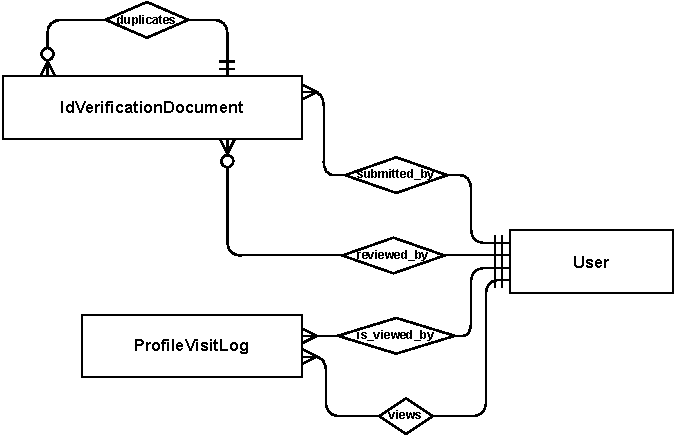
\includegraphics[width=0.78\textwidth]{image/ERD/ERD-ERD5.drawio.pdf}
    \caption{Identity Verification \& Profile Visits ERD}
    \label{fig:erd-identity-verification--profile-visits}
\end{figure}

\Needspace{8\baselineskip}
\paragraph*{b) Table of entities}\nopagebreak[4]
\begin{center}\nopagebreak[4]
\small\sloppy
\begin{longtable}{|L{2.5cm}|L{9.5cm}|}
\hline
\rowcolor{fptHeader}\textbf{Entity} & \textbf{Fields and descriptions} \\* \hline
\endfirsthead
\hline
\rowcolor{fptHeader}\textbf{Entity} & \textbf{Fields and descriptions} \\* \hline
\endhead
\hline\endfoot
\endlastfoot
\texttt{User} & - id: used to store the unique identifier of the record \\*
& - email: used to store the account email address \\
& - password: used to store the hashed account password \\
& - is\allowbreak Banned: used to store whether the account is banned \\
& - created\allowbreak At: used to store the creation timestamp \\
& - updated\allowbreak At: used to store the last update timestamp \\
& - deleted\allowbreak At: used to store the soft-deletion timestamp \\
& - stripe\allowbreak Customer\allowbreak Id: used to store the stripe customer id text value \\
& - stripe\allowbreak Account\allowbreak Id: used to store the stripe account id text value \\
& - stripe\allowbreak Onboarding\allowbreak Completed: used to store whether Stripe onboarding is completed \\
& - role\allowbreak Id: used to store the foreign key reference to the primary role \\ \hline
\texttt{Id\allowbreak Verification\allowbreak Document} & - id: used to store the unique identifier of the record \\*
& - user\allowbreak Id: used to store the foreign key reference to the user \\
& - document\allowbreak Type: used to store the document type value from the DocumentType enumeration \\
& - file\allowbreak Url: used to store the file URL \\
& - status: used to store the status value from the VerificationStatus enumeration \\
& - admin\allowbreak Id: used to store the foreign key reference to the reviewing administrator \\
& - review\allowbreak Notes: used to store the review notes text \\
& - created\allowbreak At: used to store the creation timestamp \\
& - reviewed\allowbreak At: used to store the review timestamp \\
& - deleted\allowbreak At: used to store the soft-deletion timestamp \\
& - ai\allowbreak Status: used to store the ai status text value \\
& - ai\allowbreak Score: used to store the AI verification score \\
& - ai\allowbreak Summary: used to store the AI summary data in JSON format \\
& - ai\allowbreak Selfie\allowbreak Summary: used to store the AI selfie summary data in JSON format \\
& - ai\allowbreak Error: used to store the ai error text value \\
& - ai\allowbreak Scanned\allowbreak At: used to store the AI scan timestamp \\
& - back\allowbreak File\allowbreak Url: used to store the back side file URL \\
& - identity\allowbreak Number: used to store the identity document number \\
& - duplicate\allowbreak Of\allowbreak Id: used to store the foreign key reference to the duplicate document \\ \hline
\texttt{Profile\allowbreak Visit\allowbreak Log} & - id: used to store the unique identifier of the record \\*
& - viewer\allowbreak Id: used to store the foreign key reference to the viewing user \\
& - target\allowbreak Freelancer\allowbreak Id: used to store the foreign key reference to the target freelancer \\
& - viewed\allowbreak At: used to store the view timestamp \\ \hline
\end{longtable}
\end{center}

% ===============================================
% 4.1.5.7 ERD6
% ===============================================
\Needspace{12\baselineskip}
\paragraph{Portfolio \& Skills}

This ERD describes the Portfolio \& Skills module. It stores portfolio items, freelancer skills, skill catalog, and portfolio likes. These tables support portfolio management, skill catalog, skill proficiency, and liking portfolios.

\Needspace{12\baselineskip}
\paragraph*{a) ERD}
\begin{figure}[H]
    \centering
    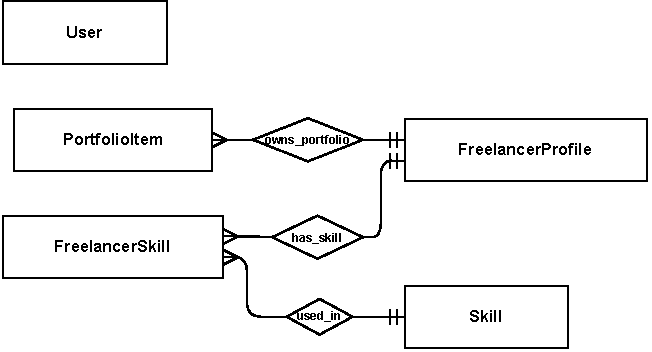
\includegraphics[width=0.78\textwidth]{image/ERD/ERD-ERD6.drawio.pdf}
    \caption{Portfolio \& Skills ERD}
    \label{fig:erd-portfolio--skills}
\end{figure}

\Needspace{8\baselineskip}
\paragraph*{b) Table of entities}\nopagebreak[4]
\begin{center}\nopagebreak[4]
\small\sloppy
\begin{longtable}{|L{2.5cm}|L{9.5cm}|}
\hline
\rowcolor{fptHeader}\textbf{Entity} & \textbf{Fields and descriptions} \\* \hline
\endfirsthead
\hline
\rowcolor{fptHeader}\textbf{Entity} & \textbf{Fields and descriptions} \\* \hline
\endhead
\hline\endfoot
\endlastfoot
\texttt{User} & - id: used to store the unique identifier of the record \\*
& - email: used to store the account email address \\
& - password: used to store the hashed account password \\
& - is\allowbreak Banned: used to store whether the account is banned \\
& - created\allowbreak At: used to store the creation timestamp \\
& - updated\allowbreak At: used to store the last update timestamp \\
& - deleted\allowbreak At: used to store the soft-deletion timestamp \\
& - stripe\allowbreak Customer\allowbreak Id: used to store the stripe customer id text value \\
& - stripe\allowbreak Account\allowbreak Id: used to store the stripe account id text value \\
& - stripe\allowbreak Onboarding\allowbreak Completed: used to store whether Stripe onboarding is completed \\
& - role\allowbreak Id: used to store the foreign key reference to the primary role \\ \hline
\texttt{Freelancer\allowbreak Profile} & - id: used to store the unique identifier of the record \\*
& - profile\allowbreak Id: used to store the foreign key reference to the profile \\
& - title: used to store the title text \\
& - education: used to store the list of education \\
& - certifications: used to store the list of certifications \\
& - languages: used to store the list of languages \\
& - cv\allowbreak Url: used to store the uploaded CV file URL \\
& - cv\allowbreak File\allowbreak Name: used to store the cv file name text value \\
& - cv\allowbreak Public\allowbreak Id: used to store the cv public id text value \\
& - cv\allowbreak Uploaded\allowbreak At: used to store the cv uploaded at timestamp \\
& - experience: used to store the list of experience \\
& - id\allowbreak Verified: used to store whether the identity is verified \\
& - created\allowbreak At: used to store the creation timestamp \\
& - updated\allowbreak At: used to store the last update timestamp \\ \hline
\texttt{Freelancer\allowbreak Skill} & - id: used to store the unique identifier of the record \\*
& - freelancer\allowbreak Profile\allowbreak Id: used to store the foreign key reference to the freelancer profile \\
& - skill\allowbreak Id: used to store the foreign key reference to the skill \\
& - proficiency\allowbreak Level: used to store the skill proficiency level \\ \hline
\texttt{Skill} & - id: used to store the unique identifier of the record \\*
& - name: used to store the name value \\
& - slug: used to store the URL slug \\
& - description: used to store the description text \\
& - deleted\allowbreak At: used to store the soft-deletion timestamp \\
& - created\allowbreak At: used to store the creation timestamp \\
& - updated\allowbreak At: used to store the last update timestamp \\ \hline
\texttt{Portfolio\allowbreak Item} & - id: used to store the unique identifier of the record \\*
& - freelancer\allowbreak Profile\allowbreak Id: used to store the foreign key reference to the freelancer profile \\
& - title: used to store the title text \\
& - description: used to store the description text \\
& - technologies: used to store the list of technologies \\
& - project\allowbreak Url: used to store the project URL \\
& - source: used to store the source value from the ProfileContentSource enumeration \\
& - created\allowbreak At: used to store the creation timestamp \\
& - updated\allowbreak At: used to store the last update timestamp \\
& - deleted\allowbreak At: used to store the soft-deletion timestamp \\ \hline
\texttt{Portfolio\allowbreak Like} & - user\allowbreak Id: used to store the foreign key reference to the user \\*
& - portfolio\allowbreak Item\allowbreak Id: used to store the foreign key reference to the portfolio item \\
& - created\allowbreak At: used to store the creation timestamp \\ \hline
\end{longtable}
\end{center}

% ===============================================
% 4.1.5.8 ERD7
% ===============================================
\Needspace{12\baselineskip}
\paragraph{Favorites \& Follows}

This ERD describes the Favorites \& Follows module. It stores favorite freelancer and follow relationships. These tables support bookmarking favorite freelancers and following/unfollowing.

\Needspace{12\baselineskip}
\paragraph*{a) ERD}
\begin{figure}[H]
    \centering
    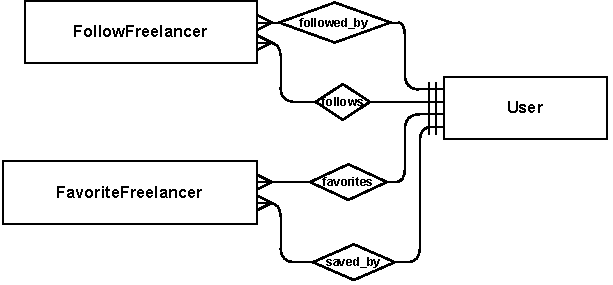
\includegraphics[width=0.78\textwidth]{image/ERD/ERD-ERD7.drawio.pdf}
    \caption{Favorites \& Follows ERD}
    \label{fig:erd-favorites--follows}
\end{figure}

\Needspace{8\baselineskip}
\paragraph*{b) Table of entities}\nopagebreak[4]
\begin{center}\nopagebreak[4]
\small\sloppy
\begin{longtable}{|L{2.5cm}|L{9.5cm}|}
\hline
\rowcolor{fptHeader}\textbf{Entity} & \textbf{Fields and descriptions} \\* \hline
\endfirsthead
\hline
\rowcolor{fptHeader}\textbf{Entity} & \textbf{Fields and descriptions} \\* \hline
\endhead
\hline\endfoot
\endlastfoot
\texttt{User} & - id: used to store the unique identifier of the record \\*
& - email: used to store the account email address \\
& - password: used to store the hashed account password \\
& - is\allowbreak Banned: used to store whether the account is banned \\
& - created\allowbreak At: used to store the creation timestamp \\
& - updated\allowbreak At: used to store the last update timestamp \\
& - deleted\allowbreak At: used to store the soft-deletion timestamp \\
& - stripe\allowbreak Customer\allowbreak Id: used to store the stripe customer id text value \\
& - stripe\allowbreak Account\allowbreak Id: used to store the stripe account id text value \\
& - stripe\allowbreak Onboarding\allowbreak Completed: used to store whether Stripe onboarding is completed \\
& - role\allowbreak Id: used to store the foreign key reference to the primary role \\ \hline
\texttt{Favorite\allowbreak Freelancer} & - client\allowbreak Id: used to store the foreign key reference to the client \\*
& - freelancer\allowbreak Id: used to store the foreign key reference to the freelancer \\
& - created\allowbreak At: used to store the creation timestamp \\ \hline
\texttt{Follow\allowbreak Freelancer} & - client\allowbreak Id: used to store the foreign key reference to the client \\*
& - freelancer\allowbreak Id: used to store the foreign key reference to the freelancer \\
& - created\allowbreak At: used to store the creation timestamp \\ \hline
\end{longtable}
\end{center}

% ===============================================
% 4.1.5.9 ERD8
% ===============================================
\Needspace{12\baselineskip}
\paragraph{Job Posting}

This ERD describes the Job Posting module. It stores job categories, jobs, job-category links, and job-skill links. These tables support creating, editing, publishing, closing, and categorizing jobs.

\Needspace{12\baselineskip}
\paragraph*{a) ERD}
\begin{figure}[H]
    \centering
    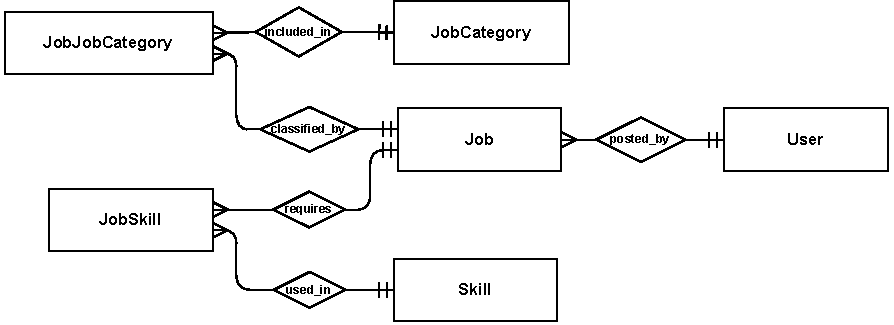
\includegraphics[width=0.78\textwidth]{image/ERD/ERD-ERD8.drawio.pdf}
    \caption{Job Posting ERD}
    \label{fig:erd-job-posting}
\end{figure}

\Needspace{8\baselineskip}
\paragraph*{b) Table of entities}\nopagebreak[4]
\begin{center}\nopagebreak[4]
\small\sloppy
\begin{longtable}{|L{2.5cm}|L{9.5cm}|}
\hline
\rowcolor{fptHeader}\textbf{Entity} & \textbf{Fields and descriptions} \\* \hline
\endfirsthead
\hline
\rowcolor{fptHeader}\textbf{Entity} & \textbf{Fields and descriptions} \\* \hline
\endhead
\hline\endfoot
\endlastfoot
\texttt{User} & - id: used to store the unique identifier of the record \\*
& - email: used to store the account email address \\
& - password: used to store the hashed account password \\
& - is\allowbreak Banned: used to store whether the account is banned \\
& - created\allowbreak At: used to store the creation timestamp \\
& - updated\allowbreak At: used to store the last update timestamp \\
& - deleted\allowbreak At: used to store the soft-deletion timestamp \\
& - stripe\allowbreak Customer\allowbreak Id: used to store the stripe customer id text value \\
& - stripe\allowbreak Account\allowbreak Id: used to store the stripe account id text value \\
& - stripe\allowbreak Onboarding\allowbreak Completed: used to store whether Stripe onboarding is completed \\
& - role\allowbreak Id: used to store the foreign key reference to the primary role \\ \hline
\texttt{Job} & - id: used to store the unique identifier of the record \\*
& - client\allowbreak Id: used to store the foreign key reference to the client \\
& - title: used to store the title text \\
& - slug: used to store the URL slug \\
& - description: used to store the description text \\
& - budget\allowbreak Min: used to store the minimum budget amount \\
& - budget\allowbreak Max: used to store the maximum budget amount \\
& - budget\allowbreak Type: used to store the budget type value from the BudgetType enumeration \\
& - deadline: used to store the deadline timestamp \\
& - status: used to store the status value from the JobStatus enumeration \\
& - expiry\allowbreak Date: used to store the expiry date timestamp \\
& - created\allowbreak At: used to store the creation timestamp \\
& - updated\allowbreak At: used to store the last update timestamp \\
& - deleted\allowbreak At: used to store the soft-deletion timestamp \\
& - hiring\allowbreak Type: used to store the hiring type value from the HiringType enumeration \\
& - positions\allowbreak Required: used to store the required number of positions \\
& - positions\allowbreak Filled: used to store the filled number of positions \\ \hline
\texttt{Job\allowbreak Category} & - id: used to store the unique identifier of the record \\*
& - name: used to store the name value \\
& - slug: used to store the URL slug \\
& - description: used to store the description text \\
& - status: used to store the status value from the JobCategoryStatus enumeration \\
& - deleted\allowbreak At: used to store the soft-deletion timestamp \\
& - created\allowbreak At: used to store the creation timestamp \\
& - updated\allowbreak At: used to store the last update timestamp \\ \hline
\texttt{Job\allowbreak Job\allowbreak Category} & - job\allowbreak Id: used to store the foreign key reference to the job \\*
& - category\allowbreak Id: used to store the foreign key reference to the job category \\ \hline
\texttt{Job\allowbreak Skill} & - job\allowbreak Id: used to store the foreign key reference to the job \\*
& - skill\allowbreak Id: used to store the foreign key reference to the skill \\ \hline
\texttt{Skill} & - id: used to store the unique identifier of the record \\*
& - name: used to store the name value \\
& - slug: used to store the URL slug \\
& - description: used to store the description text \\
& - deleted\allowbreak At: used to store the soft-deletion timestamp \\
& - created\allowbreak At: used to store the creation timestamp \\
& - updated\allowbreak At: used to store the last update timestamp \\ \hline
\end{longtable}
\end{center}

% ===============================================
% 4.1.5.10 ERD9
% ===============================================
\Needspace{12\baselineskip}
\paragraph{Job Discovery \& Alerts}

This ERD describes the Job Discovery \& Alerts module. It stores job bookmarks, recently viewed jobs, saved searches, and job alerts. These tables support browsing, bookmarking, saved filters, and alert notifications.

\Needspace{12\baselineskip}
\paragraph*{a) ERD}
\begin{figure}[H]
    \centering
    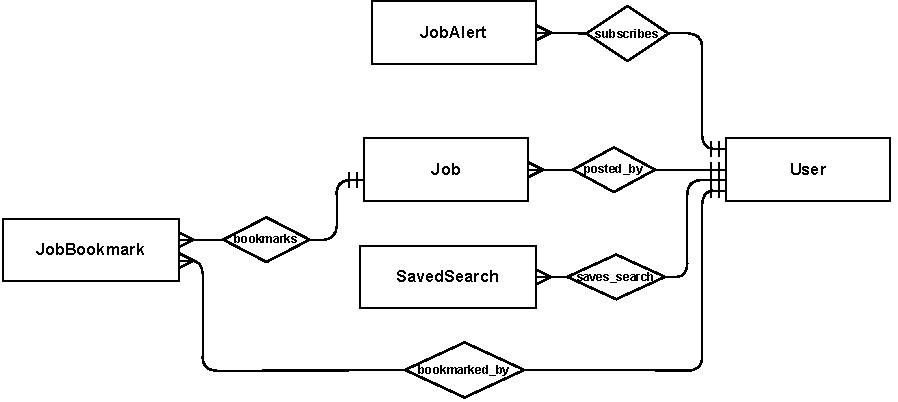
\includegraphics[width=0.78\textwidth]{image/ERD/ERD-ERD9.drawio.pdf}
    \caption{Job Discovery \& Alerts ERD}
    \label{fig:erd-job-discovery--alerts}
\end{figure}

\Needspace{8\baselineskip}
\paragraph*{b) Table of entities}\nopagebreak[4]
\begin{center}\nopagebreak[4]
\small\sloppy
\begin{longtable}{|L{2.5cm}|L{9.5cm}|}
\hline
\rowcolor{fptHeader}\textbf{Entity} & \textbf{Fields and descriptions} \\* \hline
\endfirsthead
\hline
\rowcolor{fptHeader}\textbf{Entity} & \textbf{Fields and descriptions} \\* \hline
\endhead
\hline\endfoot
\endlastfoot
\texttt{User} & - id: used to store the unique identifier of the record \\*
& - email: used to store the account email address \\
& - password: used to store the hashed account password \\
& - is\allowbreak Banned: used to store whether the account is banned \\
& - created\allowbreak At: used to store the creation timestamp \\
& - updated\allowbreak At: used to store the last update timestamp \\
& - deleted\allowbreak At: used to store the soft-deletion timestamp \\
& - stripe\allowbreak Customer\allowbreak Id: used to store the stripe customer id text value \\
& - stripe\allowbreak Account\allowbreak Id: used to store the stripe account id text value \\
& - stripe\allowbreak Onboarding\allowbreak Completed: used to store whether Stripe onboarding is completed \\
& - role\allowbreak Id: used to store the foreign key reference to the primary role \\ \hline
\texttt{Job} & - id: used to store the unique identifier of the record \\*
& - client\allowbreak Id: used to store the foreign key reference to the client \\
& - title: used to store the title text \\
& - slug: used to store the URL slug \\
& - description: used to store the description text \\
& - budget\allowbreak Min: used to store the minimum budget amount \\
& - budget\allowbreak Max: used to store the maximum budget amount \\
& - budget\allowbreak Type: used to store the budget type value from the BudgetType enumeration \\
& - deadline: used to store the deadline timestamp \\
& - status: used to store the status value from the JobStatus enumeration \\
& - expiry\allowbreak Date: used to store the expiry date timestamp \\
& - created\allowbreak At: used to store the creation timestamp \\
& - updated\allowbreak At: used to store the last update timestamp \\
& - deleted\allowbreak At: used to store the soft-deletion timestamp \\
& - hiring\allowbreak Type: used to store the hiring type value from the HiringType enumeration \\
& - positions\allowbreak Required: used to store the required number of positions \\
& - positions\allowbreak Filled: used to store the filled number of positions \\ \hline
\texttt{Job\allowbreak Bookmark} & - user\allowbreak Id: used to store the foreign key reference to the user \\*
& - job\allowbreak Id: used to store the foreign key reference to the job \\
& - created\allowbreak At: used to store the creation timestamp \\ \hline
\texttt{Recently\allowbreak Viewed\allowbreak Job} & - id: used to store the unique identifier of the record \\*
& - user\allowbreak Id: used to store the foreign key reference to the user \\
& - job\allowbreak Id: used to store the foreign key reference to the job \\
& - viewed\allowbreak At: used to store the view timestamp \\ \hline
\texttt{Saved\allowbreak Search} & - id: used to store the unique identifier of the record \\*
& - user\allowbreak Id: used to store the foreign key reference to the user \\
& - name: used to store the name value \\
& - search\allowbreak Params: used to store the saved search parameters in JSON format \\
& - created\allowbreak At: used to store the creation timestamp \\ \hline
\texttt{Job\allowbreak Alert} & - id: used to store the unique identifier of the record \\*
& - user\allowbreak Id: used to store the foreign key reference to the user \\
& - name: used to store the name value \\
& - keywords: used to store the keywords text value \\
& - skills: used to store the list of skills \\
& - frequency: used to store the frequency value from the JobAlertFrequency enumeration \\
& - channels: used to store the list of channels \\
& - is\allowbreak Active: used to store whether the record is active \\
& - last\allowbreak Sent\allowbreak At: used to store the last sent timestamp \\
& - created\allowbreak At: used to store the creation timestamp \\
& - updated\allowbreak At: used to store the last update timestamp \\ \hline
\end{longtable}
\end{center}

% ===============================================
% 4.1.5.11 ERD10
% ===============================================
\Needspace{12\baselineskip}
\paragraph{Proposal}

This ERD describes the Proposal module. It stores proposals and proposal attachments. These tables support submitting, updating, withdrawing, accepting, and rejecting proposals.

\Needspace{12\baselineskip}
\paragraph*{a) ERD}
\begin{figure}[H]
    \centering
    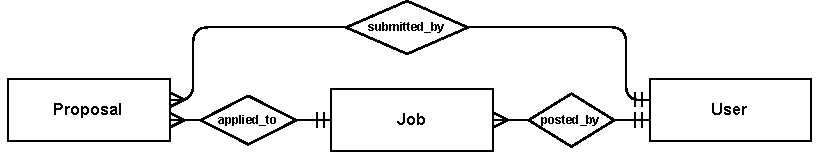
\includegraphics[width=0.78\textwidth]{image/ERD/ERD-ERD10.drawio.pdf}
    \caption{Proposal ERD}
    \label{fig:erd-proposal}
\end{figure}

\Needspace{8\baselineskip}
\paragraph*{b) Table of entities}\nopagebreak[4]
\begin{center}\nopagebreak[4]
\small\sloppy
\begin{longtable}{|L{2.5cm}|L{9.5cm}|}
\hline
\rowcolor{fptHeader}\textbf{Entity} & \textbf{Fields and descriptions} \\* \hline
\endfirsthead
\hline
\rowcolor{fptHeader}\textbf{Entity} & \textbf{Fields and descriptions} \\* \hline
\endhead
\hline\endfoot
\endlastfoot
\texttt{Job} & - id: used to store the unique identifier of the record \\*
& - client\allowbreak Id: used to store the foreign key reference to the client \\
& - title: used to store the title text \\
& - slug: used to store the URL slug \\
& - description: used to store the description text \\
& - budget\allowbreak Min: used to store the minimum budget amount \\
& - budget\allowbreak Max: used to store the maximum budget amount \\
& - budget\allowbreak Type: used to store the budget type value from the BudgetType enumeration \\
& - deadline: used to store the deadline timestamp \\
& - status: used to store the status value from the JobStatus enumeration \\
& - expiry\allowbreak Date: used to store the expiry date timestamp \\
& - created\allowbreak At: used to store the creation timestamp \\
& - updated\allowbreak At: used to store the last update timestamp \\
& - deleted\allowbreak At: used to store the soft-deletion timestamp \\
& - hiring\allowbreak Type: used to store the hiring type value from the HiringType enumeration \\
& - positions\allowbreak Required: used to store the required number of positions \\
& - positions\allowbreak Filled: used to store the filled number of positions \\ \hline
\texttt{User} & - id: used to store the unique identifier of the record \\*
& - email: used to store the account email address \\
& - password: used to store the hashed account password \\
& - is\allowbreak Banned: used to store whether the account is banned \\
& - created\allowbreak At: used to store the creation timestamp \\
& - updated\allowbreak At: used to store the last update timestamp \\
& - deleted\allowbreak At: used to store the soft-deletion timestamp \\
& - stripe\allowbreak Customer\allowbreak Id: used to store the stripe customer id text value \\
& - stripe\allowbreak Account\allowbreak Id: used to store the stripe account id text value \\
& - stripe\allowbreak Onboarding\allowbreak Completed: used to store whether Stripe onboarding is completed \\
& - role\allowbreak Id: used to store the foreign key reference to the primary role \\ \hline
\texttt{Proposal} & - id: used to store the unique identifier of the record \\*
& - job\allowbreak Id: used to store the foreign key reference to the job \\
& - freelancer\allowbreak Id: used to store the foreign key reference to the freelancer \\
& - cover\allowbreak Letter: used to store the proposal cover letter text \\
& - bid\allowbreak Amount: used to store the bid amount \\
& - delivery\allowbreak Days: used to store the delivery days integer value \\
& - status: used to store the status value from the ProposalStatus enumeration \\
& - created\allowbreak At: used to store the creation timestamp \\
& - submitted\allowbreak At: used to store the submission timestamp \\
& - accepted\allowbreak At: used to store the acceptance timestamp \\
& - rejected\allowbreak At: used to store the rejection timestamp \\
& - withdrawn\allowbreak At: used to store the withdrawal timestamp \\
& - expires\allowbreak At: used to store the expiration timestamp \\
& - updated\allowbreak At: used to store the last update timestamp \\
& - deleted\allowbreak At: used to store the soft-deletion timestamp \\ \hline
\texttt{Proposal\allowbreak Attachment} & - id: used to store the unique identifier of the record \\*
& - proposal\allowbreak Id: used to store the foreign key reference to the proposal \\
& - file\allowbreak Url: used to store the file URL \\
& - file\allowbreak Name: used to store the uploaded file name \\
& - file\allowbreak Size: used to store the file size in bytes \\
& - mime\allowbreak Type: used to store the file MIME type \\
& - created\allowbreak At: used to store the creation timestamp \\
& - deleted\allowbreak At: used to store the soft-deletion timestamp \\ \hline
\end{longtable}
\end{center}

% ===============================================
% 4.1.5.12 ERD11
% ===============================================
\Needspace{12\baselineskip}
\paragraph{Contract}

This ERD describes the Contract module. It stores contracts and contract term templates. These tables support contract creation, signing, cancellation, terms, and status management.

\Needspace{12\baselineskip}
\paragraph*{a) ERD}
\begin{figure}[H]
    \centering
    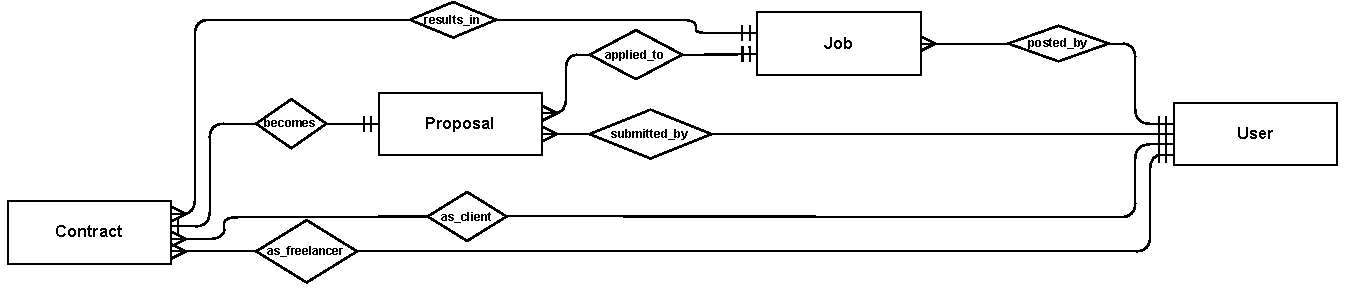
\includegraphics[width=0.78\textwidth]{image/ERD/ERD-ERD11.drawio.pdf}
    \caption{Contract ERD}
    \label{fig:erd-contract}
\end{figure}

\Needspace{8\baselineskip}
\paragraph*{b) Table of entities}\nopagebreak[4]
\begin{center}\nopagebreak[4]
\small\sloppy
\begin{longtable}{|L{2.5cm}|L{9.5cm}|}
\hline
\rowcolor{fptHeader}\textbf{Entity} & \textbf{Fields and descriptions} \\* \hline
\endfirsthead
\hline
\rowcolor{fptHeader}\textbf{Entity} & \textbf{Fields and descriptions} \\* \hline
\endhead
\hline\endfoot
\endlastfoot
\texttt{Job} & - id: used to store the unique identifier of the record \\*
& - client\allowbreak Id: used to store the foreign key reference to the client \\
& - title: used to store the title text \\
& - slug: used to store the URL slug \\
& - description: used to store the description text \\
& - budget\allowbreak Min: used to store the minimum budget amount \\
& - budget\allowbreak Max: used to store the maximum budget amount \\
& - budget\allowbreak Type: used to store the budget type value from the BudgetType enumeration \\
& - deadline: used to store the deadline timestamp \\
& - status: used to store the status value from the JobStatus enumeration \\
& - expiry\allowbreak Date: used to store the expiry date timestamp \\
& - created\allowbreak At: used to store the creation timestamp \\
& - updated\allowbreak At: used to store the last update timestamp \\
& - deleted\allowbreak At: used to store the soft-deletion timestamp \\
& - hiring\allowbreak Type: used to store the hiring type value from the HiringType enumeration \\
& - positions\allowbreak Required: used to store the required number of positions \\
& - positions\allowbreak Filled: used to store the filled number of positions \\ \hline
\texttt{Proposal} & - id: used to store the unique identifier of the record \\*
& - job\allowbreak Id: used to store the foreign key reference to the job \\
& - freelancer\allowbreak Id: used to store the foreign key reference to the freelancer \\
& - cover\allowbreak Letter: used to store the proposal cover letter text \\
& - bid\allowbreak Amount: used to store the bid amount \\
& - delivery\allowbreak Days: used to store the delivery days integer value \\
& - status: used to store the status value from the ProposalStatus enumeration \\
& - created\allowbreak At: used to store the creation timestamp \\
& - submitted\allowbreak At: used to store the submission timestamp \\
& - accepted\allowbreak At: used to store the acceptance timestamp \\
& - rejected\allowbreak At: used to store the rejection timestamp \\
& - withdrawn\allowbreak At: used to store the withdrawal timestamp \\
& - expires\allowbreak At: used to store the expiration timestamp \\
& - updated\allowbreak At: used to store the last update timestamp \\
& - deleted\allowbreak At: used to store the soft-deletion timestamp \\ \hline
\texttt{User} & - id: used to store the unique identifier of the record \\*
& - email: used to store the account email address \\
& - password: used to store the hashed account password \\
& - is\allowbreak Banned: used to store whether the account is banned \\
& - created\allowbreak At: used to store the creation timestamp \\
& - updated\allowbreak At: used to store the last update timestamp \\
& - deleted\allowbreak At: used to store the soft-deletion timestamp \\
& - stripe\allowbreak Customer\allowbreak Id: used to store the stripe customer id text value \\
& - stripe\allowbreak Account\allowbreak Id: used to store the stripe account id text value \\
& - stripe\allowbreak Onboarding\allowbreak Completed: used to store whether Stripe onboarding is completed \\
& - role\allowbreak Id: used to store the foreign key reference to the primary role \\ \hline
\texttt{Contract} & - id: used to store the unique identifier of the record \\*
& - slug: used to store the URL slug \\
& - job\allowbreak Id: used to store the foreign key reference to the job \\
& - proposal\allowbreak Id: used to store the foreign key reference to the proposal \\
& - client\allowbreak Id: used to store the foreign key reference to the client \\
& - freelancer\allowbreak Id: used to store the foreign key reference to the freelancer \\
& - terms: used to store the contract terms text \\
& - total\allowbreak Amount: used to store the total amount \\
& - status: used to store the status value from the ContractStatus enumeration \\
& - signed\allowbreak By\allowbreak Client: used to store whether the contract is signed by the client \\
& - signed\allowbreak By\allowbreak Freelancer: used to store whether the contract is signed by the freelancer \\
& - client\allowbreak Signed\allowbreak At: used to store the client signing timestamp \\
& - freelancer\allowbreak Signed\allowbreak At: used to store the freelancer signing timestamp \\
& - client\allowbreak Platform\allowbreak Fee: used to store the client platform fee amount \\
& - platform\allowbreak Fee: used to store the platform fee amount \\
& - platform\allowbreak Fee\allowbreak Status: used to store the platform fee status value from the PlatformFeeStatus enumeration \\
& - platform\allowbreak Fee\allowbreak Paid\allowbreak At: used to store the platform fee payment timestamp \\
& - client\allowbreak Fee\allowbreak Status: used to store the client fee status value from the PlatformFeeStatus enumeration \\
& - client\allowbreak Fee\allowbreak Paid\allowbreak At: used to store the client fee payment timestamp \\
& - freelancer\allowbreak Fee\allowbreak Status: used to store the freelancer fee status value from the PlatformFeeStatus enumeration \\
& - freelancer\allowbreak Fee\allowbreak Paid\allowbreak At: used to store the freelancer fee payment timestamp \\
& - hold\allowbreak Payment\allowbreak Intent\allowbreak Id: used to store the hold payment intent id text value \\
& - hold\allowbreak Milestone\allowbreak Ids: used to store the list of hold milestone ids \\
& - rejected\allowbreak At: used to store the rejection timestamp \\
& - reject\allowbreak Reason: used to store the rejection reason text \\
& - created\allowbreak At: used to store the creation timestamp \\
& - signed\allowbreak At: used to store the signing timestamp \\
& - completed\allowbreak At: used to store the completion timestamp \\
& - expires\allowbreak At: used to store the expiration timestamp \\
& - deleted\allowbreak At: used to store the soft-deletion timestamp \\ \hline
\texttt{Contract\allowbreak Term\allowbreak Template} & - id: used to store the unique identifier of the record \\*
& - creator\allowbreak Id: used to store the foreign key reference to the user \\
& - title: used to store the title text \\
& - content: used to store the content text \\
& - category: used to store the category text value \\
& - is\allowbreak Active: used to store whether the record is active \\
& - created\allowbreak At: used to store the creation timestamp \\
& - updated\allowbreak At: used to store the last update timestamp \\
& - deleted\allowbreak At: used to store the soft-deletion timestamp \\ \hline
\end{longtable}
\end{center}

% ===============================================
% 4.1.5.13 ERD12
% ===============================================
\Needspace{12\baselineskip}
\paragraph{Milestone \& Project Progress}

This ERD describes the Milestone \& Project Progress module. It stores milestones and project progress updates. These tables support milestone creation, updates, progress tracking, and client/freelancer collaboration.

\Needspace{12\baselineskip}
\paragraph*{a) ERD}
\begin{figure}[H]
    \centering
    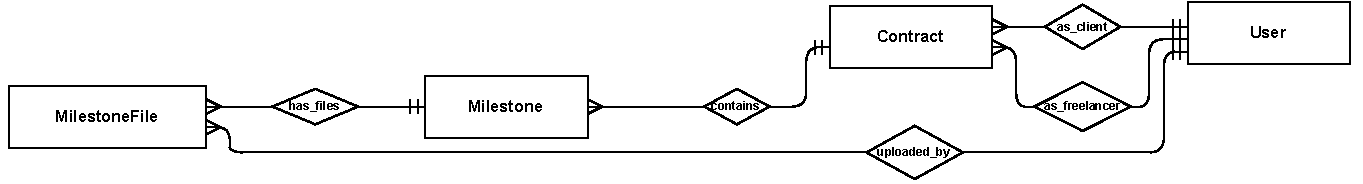
\includegraphics[width=0.78\textwidth]{image/ERD/ERD-ERD12.drawio.pdf}
    \caption{Milestone \& Project Progress ERD}
    \label{fig:erd-milestone--project-progress}
\end{figure}

\Needspace{8\baselineskip}
\paragraph*{b) Table of entities}\nopagebreak[4]
\begin{center}\nopagebreak[4]
\small\sloppy
\begin{longtable}{|L{2.5cm}|L{9.5cm}|}
\hline
\rowcolor{fptHeader}\textbf{Entity} & \textbf{Fields and descriptions} \\* \hline
\endfirsthead
\hline
\rowcolor{fptHeader}\textbf{Entity} & \textbf{Fields and descriptions} \\* \hline
\endhead
\hline\endfoot
\endlastfoot
\texttt{User} & - id: used to store the unique identifier of the record \\*
& - email: used to store the account email address \\
& - password: used to store the hashed account password \\
& - is\allowbreak Banned: used to store whether the account is banned \\
& - created\allowbreak At: used to store the creation timestamp \\
& - updated\allowbreak At: used to store the last update timestamp \\
& - deleted\allowbreak At: used to store the soft-deletion timestamp \\
& - stripe\allowbreak Customer\allowbreak Id: used to store the stripe customer id text value \\
& - stripe\allowbreak Account\allowbreak Id: used to store the stripe account id text value \\
& - stripe\allowbreak Onboarding\allowbreak Completed: used to store whether Stripe onboarding is completed \\
& - role\allowbreak Id: used to store the foreign key reference to the primary role \\ \hline
\texttt{Contract} & - id: used to store the unique identifier of the record \\*
& - slug: used to store the URL slug \\
& - job\allowbreak Id: used to store the foreign key reference to the job \\
& - proposal\allowbreak Id: used to store the foreign key reference to the proposal \\
& - client\allowbreak Id: used to store the foreign key reference to the client \\
& - freelancer\allowbreak Id: used to store the foreign key reference to the freelancer \\
& - terms: used to store the contract terms text \\
& - total\allowbreak Amount: used to store the total amount \\
& - status: used to store the status value from the ContractStatus enumeration \\
& - signed\allowbreak By\allowbreak Client: used to store whether the contract is signed by the client \\
& - signed\allowbreak By\allowbreak Freelancer: used to store whether the contract is signed by the freelancer \\
& - client\allowbreak Signed\allowbreak At: used to store the client signing timestamp \\
& - freelancer\allowbreak Signed\allowbreak At: used to store the freelancer signing timestamp \\
& - client\allowbreak Platform\allowbreak Fee: used to store the client platform fee amount \\
& - platform\allowbreak Fee: used to store the platform fee amount \\
& - platform\allowbreak Fee\allowbreak Status: used to store the platform fee status value from the PlatformFeeStatus enumeration \\
& - platform\allowbreak Fee\allowbreak Paid\allowbreak At: used to store the platform fee payment timestamp \\
& - client\allowbreak Fee\allowbreak Status: used to store the client fee status value from the PlatformFeeStatus enumeration \\
& - client\allowbreak Fee\allowbreak Paid\allowbreak At: used to store the client fee payment timestamp \\
& - freelancer\allowbreak Fee\allowbreak Status: used to store the freelancer fee status value from the PlatformFeeStatus enumeration \\
& - freelancer\allowbreak Fee\allowbreak Paid\allowbreak At: used to store the freelancer fee payment timestamp \\
& - hold\allowbreak Payment\allowbreak Intent\allowbreak Id: used to store the hold payment intent id text value \\
& - hold\allowbreak Milestone\allowbreak Ids: used to store the list of hold milestone ids \\
& - rejected\allowbreak At: used to store the rejection timestamp \\
& - reject\allowbreak Reason: used to store the rejection reason text \\
& - created\allowbreak At: used to store the creation timestamp \\
& - signed\allowbreak At: used to store the signing timestamp \\
& - completed\allowbreak At: used to store the completion timestamp \\
& - expires\allowbreak At: used to store the expiration timestamp \\
& - deleted\allowbreak At: used to store the soft-deletion timestamp \\ \hline
\texttt{Milestone} & - id: used to store the unique identifier of the record \\*
& - contract\allowbreak Id: used to store the foreign key reference to the contract \\
& - title: used to store the title text \\
& - description: used to store the description text \\
& - amount: used to store the amount value \\
& - status: used to store the status value from the MilestoneStatus enumeration \\
& - payment\allowbreak Status: used to store the payment status value from the MilestonePaymentStatus enumeration \\
& - due\allowbreak Date: used to store the due date timestamp \\
& - completed\allowbreak At: used to store the completion timestamp \\
& - created\allowbreak At: used to store the creation timestamp \\
& - updated\allowbreak At: used to store the last update timestamp \\
& - deleted\allowbreak At: used to store the soft-deletion timestamp \\ \hline
\texttt{Milestone\allowbreak File} & - id: used to store the unique identifier of the record \\*
& - milestone\allowbreak Id: used to store the foreign key reference to the milestone \\
& - uploader\allowbreak Id: used to store the foreign key reference to the uploading user \\
& - file\allowbreak Url: used to store the file URL \\
& - public\allowbreak Id: used to store the Cloudinary public identifier \\
& - file\allowbreak Name: used to store the uploaded file name \\
& - created\allowbreak At: used to store the creation timestamp \\
& - deleted\allowbreak At: used to store the soft-deletion timestamp \\ \hline
\texttt{Project\allowbreak Progress\allowbreak Update} & - id: used to store the unique identifier of the record \\*
& - contract\allowbreak Id: used to store the foreign key reference to the contract \\
& - freelancer\allowbreak Id: used to store the foreign key reference to the freelancer \\
& - note: used to store the progress note text \\
& - updated\allowbreak At: used to store the last update timestamp \\ \hline
\end{longtable}
\end{center}

% ===============================================
% 4.1.5.14 ERD13
% ===============================================
\Needspace{12\baselineskip}
\paragraph{Milestone Submission}

This ERD describes the Milestone Submission module. It stores milestone files, submissions, and submission files. These tables support uploading deliverables, submitting milestones, and reviewing submissions.

\Needspace{12\baselineskip}
\paragraph*{a) ERD}
\begin{figure}[H]
    \centering
    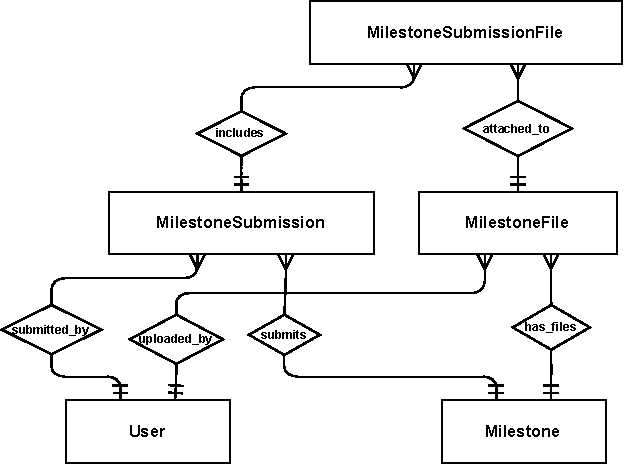
\includegraphics[width=0.78\textwidth]{image/ERD/ERD-ERD13.drawio.pdf}
    \caption{Milestone Submission ERD}
    \label{fig:erd-milestone-submission}
\end{figure}

\Needspace{8\baselineskip}
\paragraph*{b) Table of entities}\nopagebreak[4]
\begin{center}\nopagebreak[4]
\small\sloppy
\begin{longtable}{|L{2.5cm}|L{9.5cm}|}
\hline
\rowcolor{fptHeader}\textbf{Entity} & \textbf{Fields and descriptions} \\* \hline
\endfirsthead
\hline
\rowcolor{fptHeader}\textbf{Entity} & \textbf{Fields and descriptions} \\* \hline
\endhead
\hline\endfoot
\endlastfoot
\texttt{User} & - id: used to store the unique identifier of the record \\*
& - email: used to store the account email address \\
& - password: used to store the hashed account password \\
& - is\allowbreak Banned: used to store whether the account is banned \\
& - created\allowbreak At: used to store the creation timestamp \\
& - updated\allowbreak At: used to store the last update timestamp \\
& - deleted\allowbreak At: used to store the soft-deletion timestamp \\
& - stripe\allowbreak Customer\allowbreak Id: used to store the stripe customer id text value \\
& - stripe\allowbreak Account\allowbreak Id: used to store the stripe account id text value \\
& - stripe\allowbreak Onboarding\allowbreak Completed: used to store whether Stripe onboarding is completed \\
& - role\allowbreak Id: used to store the foreign key reference to the primary role \\ \hline
\texttt{Milestone} & - id: used to store the unique identifier of the record \\*
& - contract\allowbreak Id: used to store the foreign key reference to the contract \\
& - title: used to store the title text \\
& - description: used to store the description text \\
& - amount: used to store the amount value \\
& - status: used to store the status value from the MilestoneStatus enumeration \\
& - payment\allowbreak Status: used to store the payment status value from the MilestonePaymentStatus enumeration \\
& - due\allowbreak Date: used to store the due date timestamp \\
& - completed\allowbreak At: used to store the completion timestamp \\
& - created\allowbreak At: used to store the creation timestamp \\
& - updated\allowbreak At: used to store the last update timestamp \\
& - deleted\allowbreak At: used to store the soft-deletion timestamp \\ \hline
\texttt{Milestone\allowbreak File} & - id: used to store the unique identifier of the record \\*
& - milestone\allowbreak Id: used to store the foreign key reference to the milestone \\
& - uploader\allowbreak Id: used to store the foreign key reference to the uploading user \\
& - file\allowbreak Url: used to store the file URL \\
& - public\allowbreak Id: used to store the Cloudinary public identifier \\
& - file\allowbreak Name: used to store the uploaded file name \\
& - created\allowbreak At: used to store the creation timestamp \\
& - deleted\allowbreak At: used to store the soft-deletion timestamp \\ \hline
\texttt{Milestone\allowbreak Submission} & - id: used to store the unique identifier of the record \\*
& - milestone\allowbreak Id: used to store the foreign key reference to the milestone \\
& - freelancer\allowbreak Id: used to store the foreign key reference to the freelancer \\
& - message: used to store the message text \\
& - links: used to store the list of links \\
& - status: used to store the status value from the SubmissionStatus enumeration \\
& - change\allowbreak Request\allowbreak Message: used to store the change request message text value \\
& - change\allowbreak Request\allowbreak Due\allowbreak Date: used to store the change request due date timestamp \\
& - submitted\allowbreak At: used to store the submission timestamp \\
& - reviewed\allowbreak At: used to store the review timestamp \\
& - created\allowbreak At: used to store the creation timestamp \\
& - updated\allowbreak At: used to store the last update timestamp \\ \hline
\texttt{Milestone\allowbreak Submission\allowbreak File} & - submission\allowbreak Id: used to store the foreign key reference to the milestone submission \\*
& - file\allowbreak Id: used to store the foreign key reference to the milestone file \\ \hline
\end{longtable}
\end{center}

% ===============================================
% 4.1.5.15 ERD14
% ===============================================
\Needspace{12\baselineskip}
\paragraph{Escrow, Payments \& Certificates}

This ERD describes the Escrow, Payments \& Certificates module. It stores invoices, certificates, and transactions. These tables support funding, releasing, refunding, platform fees, payout tracking, and completion certificates.

\Needspace{12\baselineskip}
\paragraph*{a) ERD}
\begin{figure}[H]
    \centering
    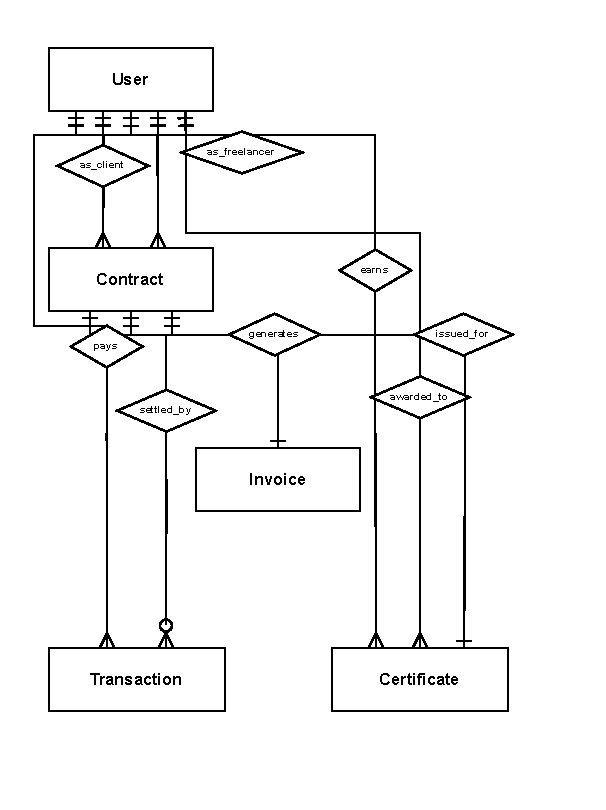
\includegraphics[width=0.78\textwidth]{image/ERD/ERD-ERD14.drawio.pdf}
    \caption{Escrow, Payments \& Certificates ERD}
    \label{fig:erd-escrow-payments--certificates}
\end{figure}

\Needspace{8\baselineskip}
\paragraph*{b) Table of entities}\nopagebreak[4]
\begin{center}\nopagebreak[4]
\small\sloppy
\begin{longtable}{|L{2.5cm}|L{9.5cm}|}
\hline
\rowcolor{fptHeader}\textbf{Entity} & \textbf{Fields and descriptions} \\* \hline
\endfirsthead
\hline
\rowcolor{fptHeader}\textbf{Entity} & \textbf{Fields and descriptions} \\* \hline
\endhead
\hline\endfoot
\endlastfoot
\texttt{User} & - id: used to store the unique identifier of the record \\*
& - email: used to store the account email address \\
& - password: used to store the hashed account password \\
& - is\allowbreak Banned: used to store whether the account is banned \\
& - created\allowbreak At: used to store the creation timestamp \\
& - updated\allowbreak At: used to store the last update timestamp \\
& - deleted\allowbreak At: used to store the soft-deletion timestamp \\
& - stripe\allowbreak Customer\allowbreak Id: used to store the stripe customer id text value \\
& - stripe\allowbreak Account\allowbreak Id: used to store the stripe account id text value \\
& - stripe\allowbreak Onboarding\allowbreak Completed: used to store whether Stripe onboarding is completed \\
& - role\allowbreak Id: used to store the foreign key reference to the primary role \\ \hline
\texttt{Contract} & - id: used to store the unique identifier of the record \\*
& - slug: used to store the URL slug \\
& - job\allowbreak Id: used to store the foreign key reference to the job \\
& - proposal\allowbreak Id: used to store the foreign key reference to the proposal \\
& - client\allowbreak Id: used to store the foreign key reference to the client \\
& - freelancer\allowbreak Id: used to store the foreign key reference to the freelancer \\
& - terms: used to store the contract terms text \\
& - total\allowbreak Amount: used to store the total amount \\
& - status: used to store the status value from the ContractStatus enumeration \\
& - signed\allowbreak By\allowbreak Client: used to store whether the contract is signed by the client \\
& - signed\allowbreak By\allowbreak Freelancer: used to store whether the contract is signed by the freelancer \\
& - client\allowbreak Signed\allowbreak At: used to store the client signing timestamp \\
& - freelancer\allowbreak Signed\allowbreak At: used to store the freelancer signing timestamp \\
& - client\allowbreak Platform\allowbreak Fee: used to store the client platform fee amount \\
& - platform\allowbreak Fee: used to store the platform fee amount \\
& - platform\allowbreak Fee\allowbreak Status: used to store the platform fee status value from the PlatformFeeStatus enumeration \\
& - platform\allowbreak Fee\allowbreak Paid\allowbreak At: used to store the platform fee payment timestamp \\
& - client\allowbreak Fee\allowbreak Status: used to store the client fee status value from the PlatformFeeStatus enumeration \\
& - client\allowbreak Fee\allowbreak Paid\allowbreak At: used to store the client fee payment timestamp \\
& - freelancer\allowbreak Fee\allowbreak Status: used to store the freelancer fee status value from the PlatformFeeStatus enumeration \\
& - freelancer\allowbreak Fee\allowbreak Paid\allowbreak At: used to store the freelancer fee payment timestamp \\
& - hold\allowbreak Payment\allowbreak Intent\allowbreak Id: used to store the hold payment intent id text value \\
& - hold\allowbreak Milestone\allowbreak Ids: used to store the list of hold milestone ids \\
& - rejected\allowbreak At: used to store the rejection timestamp \\
& - reject\allowbreak Reason: used to store the rejection reason text \\
& - created\allowbreak At: used to store the creation timestamp \\
& - signed\allowbreak At: used to store the signing timestamp \\
& - completed\allowbreak At: used to store the completion timestamp \\
& - expires\allowbreak At: used to store the expiration timestamp \\
& - deleted\allowbreak At: used to store the soft-deletion timestamp \\ \hline
\texttt{Invoice} & - id: used to store the unique identifier of the record \\*
& - contract\allowbreak Id: used to store the foreign key reference to the contract \\
& - invoice\allowbreak Number: used to store the invoice number text value \\
& - total\allowbreak Amount: used to store the total amount \\
& - description: used to store the description text \\
& - status: used to store the status value from the InvoiceStatus enumeration \\
& - issued\allowbreak At: used to store the issue timestamp \\
& - due\allowbreak Date: used to store the due date timestamp \\
& - paid\allowbreak At: used to store the payment timestamp \\
& - created\allowbreak At: used to store the creation timestamp \\
& - updated\allowbreak At: used to store the last update timestamp \\
& - deleted\allowbreak At: used to store the soft-deletion timestamp \\ \hline
\texttt{Transaction} & - id: used to store the unique identifier of the record \\*
& - user\allowbreak Id: used to store the foreign key reference to the user \\
& - contract\allowbreak Id: used to store the foreign key reference to the contract \\
& - milestone\allowbreak Id: used to store the milestone id integer value \\
& - dispute\allowbreak Id: used to store the dispute id integer value \\
& - amount: used to store the amount value \\
& - currency: used to store the currency code \\
& - type: used to store the type value from the TransactionType enumeration \\
& - status: used to store the status value from the TransactionStatus enumeration \\
& - stripe\allowbreak Payment\allowbreak Intent\allowbreak Id: used to store the stripe payment intent id text value \\
& - stripe\allowbreak Transfer\allowbreak Id: used to store the stripe transfer id text value \\
& - stripe\allowbreak Refund\allowbreak Id: used to store the stripe refund id text value \\
& - metadata: used to store the metadata in JSON format \\
& - created\allowbreak At: used to store the creation timestamp \\
& - updated\allowbreak At: used to store the last update timestamp \\ \hline
\texttt{Certificate} & - id: used to store the unique identifier of the record \\*
& - contract\allowbreak Id: used to store the foreign key reference to the contract \\
& - freelancer\allowbreak Id: used to store the foreign key reference to the freelancer \\
& - client\allowbreak Id: used to store the foreign key reference to the client \\
& - certificate\allowbreak Uid: used to store the certificate unique identifier \\
& - completion\allowbreak Date: used to store the completion date timestamp \\
& - metadata: used to store the metadata in JSON format \\
& - created\allowbreak At: used to store the creation timestamp \\ \hline
\end{longtable}
\end{center}

% ===============================================
% 4.1.5.16 ERD15
% ===============================================
\Needspace{12\baselineskip}
\paragraph{Dispute Core}

This ERD describes the Dispute Core module. It stores disputes and dispute fees. These tables support opening disputes and charging dispute fees.

\Needspace{12\baselineskip}
\paragraph*{a) ERD}
\begin{figure}[H]
    \centering
    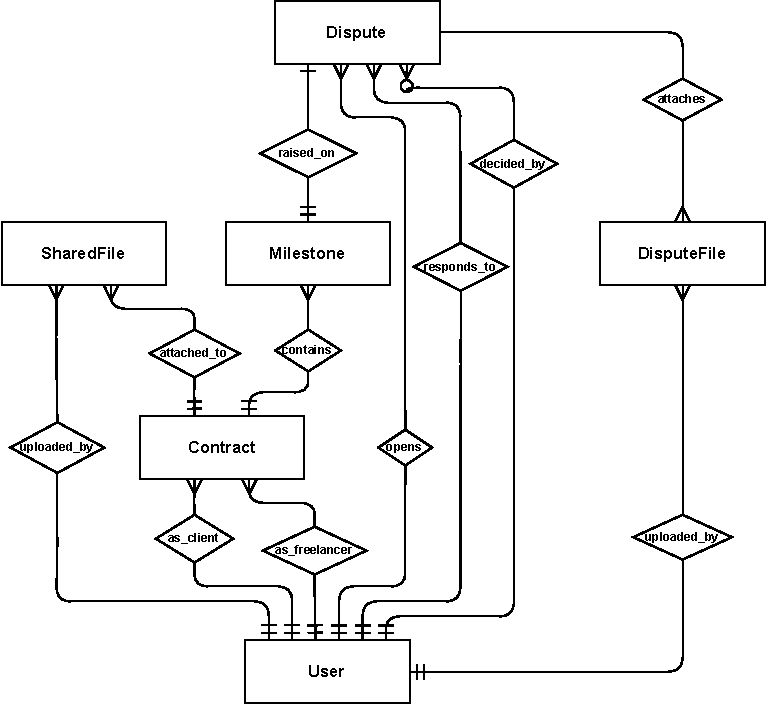
\includegraphics[width=0.78\textwidth]{image/ERD/ERD-ERD15.drawio.pdf}
    \caption{Dispute Core ERD}
    \label{fig:erd-dispute-core}
\end{figure}

\Needspace{8\baselineskip}
\paragraph*{b) Table of entities}\nopagebreak[4]
\begin{center}\nopagebreak[4]
\small\sloppy
\begin{longtable}{|L{2.5cm}|L{9.5cm}|}
\hline
\rowcolor{fptHeader}\textbf{Entity} & \textbf{Fields and descriptions} \\* \hline
\endfirsthead
\hline
\rowcolor{fptHeader}\textbf{Entity} & \textbf{Fields and descriptions} \\* \hline
\endhead
\hline\endfoot
\endlastfoot
\texttt{Contract} & - id: used to store the unique identifier of the record \\*
& - slug: used to store the URL slug \\
& - job\allowbreak Id: used to store the foreign key reference to the job \\
& - proposal\allowbreak Id: used to store the foreign key reference to the proposal \\
& - client\allowbreak Id: used to store the foreign key reference to the client \\
& - freelancer\allowbreak Id: used to store the foreign key reference to the freelancer \\
& - terms: used to store the contract terms text \\
& - total\allowbreak Amount: used to store the total amount \\
& - status: used to store the status value from the ContractStatus enumeration \\
& - signed\allowbreak By\allowbreak Client: used to store whether the contract is signed by the client \\
& - signed\allowbreak By\allowbreak Freelancer: used to store whether the contract is signed by the freelancer \\
& - client\allowbreak Signed\allowbreak At: used to store the client signing timestamp \\
& - freelancer\allowbreak Signed\allowbreak At: used to store the freelancer signing timestamp \\
& - client\allowbreak Platform\allowbreak Fee: used to store the client platform fee amount \\
& - platform\allowbreak Fee: used to store the platform fee amount \\
& - platform\allowbreak Fee\allowbreak Status: used to store the platform fee status value from the PlatformFeeStatus enumeration \\
& - platform\allowbreak Fee\allowbreak Paid\allowbreak At: used to store the platform fee payment timestamp \\
& - client\allowbreak Fee\allowbreak Status: used to store the client fee status value from the PlatformFeeStatus enumeration \\
& - client\allowbreak Fee\allowbreak Paid\allowbreak At: used to store the client fee payment timestamp \\
& - freelancer\allowbreak Fee\allowbreak Status: used to store the freelancer fee status value from the PlatformFeeStatus enumeration \\
& - freelancer\allowbreak Fee\allowbreak Paid\allowbreak At: used to store the freelancer fee payment timestamp \\
& - hold\allowbreak Payment\allowbreak Intent\allowbreak Id: used to store the hold payment intent id text value \\
& - hold\allowbreak Milestone\allowbreak Ids: used to store the list of hold milestone ids \\
& - rejected\allowbreak At: used to store the rejection timestamp \\
& - reject\allowbreak Reason: used to store the rejection reason text \\
& - created\allowbreak At: used to store the creation timestamp \\
& - signed\allowbreak At: used to store the signing timestamp \\
& - completed\allowbreak At: used to store the completion timestamp \\
& - expires\allowbreak At: used to store the expiration timestamp \\
& - deleted\allowbreak At: used to store the soft-deletion timestamp \\ \hline
\texttt{Milestone} & - id: used to store the unique identifier of the record \\*
& - contract\allowbreak Id: used to store the foreign key reference to the contract \\
& - title: used to store the title text \\
& - description: used to store the description text \\
& - amount: used to store the amount value \\
& - status: used to store the status value from the MilestoneStatus enumeration \\
& - payment\allowbreak Status: used to store the payment status value from the MilestonePaymentStatus enumeration \\
& - due\allowbreak Date: used to store the due date timestamp \\
& - completed\allowbreak At: used to store the completion timestamp \\
& - created\allowbreak At: used to store the creation timestamp \\
& - updated\allowbreak At: used to store the last update timestamp \\
& - deleted\allowbreak At: used to store the soft-deletion timestamp \\ \hline
\texttt{User} & - id: used to store the unique identifier of the record \\*
& - email: used to store the account email address \\
& - password: used to store the hashed account password \\
& - is\allowbreak Banned: used to store whether the account is banned \\
& - created\allowbreak At: used to store the creation timestamp \\
& - updated\allowbreak At: used to store the last update timestamp \\
& - deleted\allowbreak At: used to store the soft-deletion timestamp \\
& - stripe\allowbreak Customer\allowbreak Id: used to store the stripe customer id text value \\
& - stripe\allowbreak Account\allowbreak Id: used to store the stripe account id text value \\
& - stripe\allowbreak Onboarding\allowbreak Completed: used to store whether Stripe onboarding is completed \\
& - role\allowbreak Id: used to store the foreign key reference to the primary role \\ \hline
\texttt{Shared\allowbreak File} & - id: used to store the unique identifier of the record \\*
& - contract\allowbreak Id: used to store the foreign key reference to the contract \\
& - uploader\allowbreak Id: used to store the foreign key reference to the uploading user \\
& - file\allowbreak Url: used to store the file URL \\
& - public\allowbreak Id: used to store the Cloudinary public identifier \\
& - file\allowbreak Name: used to store the uploaded file name \\
& - created\allowbreak At: used to store the creation timestamp \\
& - deleted\allowbreak At: used to store the soft-deletion timestamp \\ \hline
\texttt{Dispute} & - id: used to store the unique identifier of the record \\*
& - milestone\allowbreak Id: used to store the foreign key reference to the milestone \\
& - opened\allowbreak By\allowbreak Id: used to store the foreign key reference to the user who opened the dispute \\
& - respondent\allowbreak Id: used to store the foreign key reference to the responding party \\
& - reason: used to store the reason text \\
& - description: used to store the description text \\
& - resolution\allowbreak Type: used to store the resolution type value from the DisputeResolutionType enumeration \\
& - proposed\allowbreak Freelancer\allowbreak Amount: used to store the proposed freelancer amount amount \\
& - proposed\allowbreak Client\allowbreak Amount: used to store the proposed client amount amount \\
& - proposed\allowbreak Due\allowbreak Date: used to store the proposed due date timestamp \\
& - previous\allowbreak Milestone\allowbreak Status: used to store the previous milestone status value from the MilestoneStatus enumeration \\
& - decline\allowbreak Reason: used to store the decline reason text \\
& - declined\allowbreak At: used to store the declined at timestamp \\
& - escalated\allowbreak At: used to store the escalated at timestamp \\
& - status: used to store the status value from the DisputeStatus enumeration \\
& - arbitration\allowbreak Fee: used to store the arbitration fee amount \\
& - fee\allowbreak Deadline: used to store the fee deadline timestamp \\
& - response\allowbreak Deadline: used to store the response deadline timestamp \\
& - freelancer\allowbreak Amount: used to store the freelancer amount amount \\
& - client\allowbreak Amount: used to store the client amount amount \\
& - decision\allowbreak Reason: used to store the decision reason text value \\
& - decision\allowbreak By\allowbreak Id: used to store the foreign key reference to the deciding administrator \\
& - decision\allowbreak At: used to store the decision timestamp \\
& - final\allowbreak Decision\allowbreak At: used to store the final decision timestamp \\
& - created\allowbreak At: used to store the creation timestamp \\
& - updated\allowbreak At: used to store the last update timestamp \\ \hline
\end{longtable}
\end{center}

% ===============================================
% 4.1.5.17 ERD16
% ===============================================
\Needspace{12\baselineskip}
\paragraph{Dispute Resolution}

This ERD describes the Dispute Resolution module. It stores dispute evidence and decision reviews. These tables support evidence submission and review of dispute decisions.

\Needspace{12\baselineskip}
\paragraph*{a) ERD}
\begin{figure}[H]
    \centering
    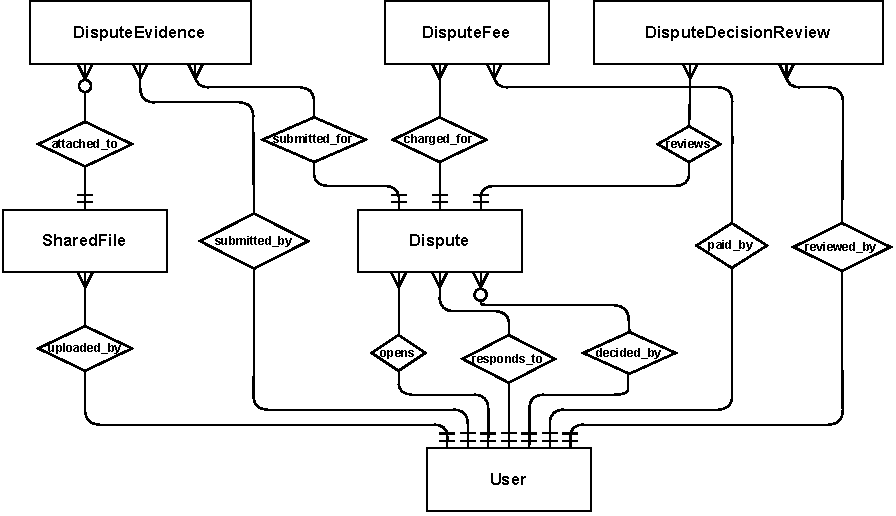
\includegraphics[width=0.78\textwidth]{image/ERD/ERD-ERD16.drawio.pdf}
    \caption{Dispute Resolution ERD}
    \label{fig:erd-dispute-resolution}
\end{figure}

\Needspace{8\baselineskip}
\paragraph*{b) Table of entities}\nopagebreak[4]
\begin{center}\nopagebreak[4]
\small\sloppy
\begin{longtable}{|L{2.5cm}|L{9.5cm}|}
\hline
\rowcolor{fptHeader}\textbf{Entity} & \textbf{Fields and descriptions} \\* \hline
\endfirsthead
\hline
\rowcolor{fptHeader}\textbf{Entity} & \textbf{Fields and descriptions} \\* \hline
\endhead
\hline\endfoot
\endlastfoot
\texttt{User} & - id: used to store the unique identifier of the record \\*
& - email: used to store the account email address \\
& - password: used to store the hashed account password \\
& - is\allowbreak Banned: used to store whether the account is banned \\
& - created\allowbreak At: used to store the creation timestamp \\
& - updated\allowbreak At: used to store the last update timestamp \\
& - deleted\allowbreak At: used to store the soft-deletion timestamp \\
& - stripe\allowbreak Customer\allowbreak Id: used to store the stripe customer id text value \\
& - stripe\allowbreak Account\allowbreak Id: used to store the stripe account id text value \\
& - stripe\allowbreak Onboarding\allowbreak Completed: used to store whether Stripe onboarding is completed \\
& - role\allowbreak Id: used to store the foreign key reference to the primary role \\ \hline
\texttt{Dispute} & - id: used to store the unique identifier of the record \\*
& - milestone\allowbreak Id: used to store the foreign key reference to the milestone \\
& - opened\allowbreak By\allowbreak Id: used to store the foreign key reference to the user who opened the dispute \\
& - respondent\allowbreak Id: used to store the foreign key reference to the responding party \\
& - reason: used to store the reason text \\
& - description: used to store the description text \\
& - resolution\allowbreak Type: used to store the resolution type value from the DisputeResolutionType enumeration \\
& - proposed\allowbreak Freelancer\allowbreak Amount: used to store the proposed freelancer amount amount \\
& - proposed\allowbreak Client\allowbreak Amount: used to store the proposed client amount amount \\
& - proposed\allowbreak Due\allowbreak Date: used to store the proposed due date timestamp \\
& - previous\allowbreak Milestone\allowbreak Status: used to store the previous milestone status value from the MilestoneStatus enumeration \\
& - decline\allowbreak Reason: used to store the decline reason text \\
& - declined\allowbreak At: used to store the declined at timestamp \\
& - escalated\allowbreak At: used to store the escalated at timestamp \\
& - status: used to store the status value from the DisputeStatus enumeration \\
& - arbitration\allowbreak Fee: used to store the arbitration fee amount \\
& - fee\allowbreak Deadline: used to store the fee deadline timestamp \\
& - response\allowbreak Deadline: used to store the response deadline timestamp \\
& - freelancer\allowbreak Amount: used to store the freelancer amount amount \\
& - client\allowbreak Amount: used to store the client amount amount \\
& - decision\allowbreak Reason: used to store the decision reason text value \\
& - decision\allowbreak By\allowbreak Id: used to store the foreign key reference to the deciding administrator \\
& - decision\allowbreak At: used to store the decision timestamp \\
& - final\allowbreak Decision\allowbreak At: used to store the final decision timestamp \\
& - created\allowbreak At: used to store the creation timestamp \\
& - updated\allowbreak At: used to store the last update timestamp \\ \hline
\texttt{Dispute\allowbreak Fee} & - id: used to store the unique identifier of the record \\*
& - dispute\allowbreak Id: used to store the foreign key reference to the dispute \\
& - user\allowbreak Id: used to store the foreign key reference to the user \\
& - amount: used to store the amount value \\
& - status: used to store the status value from the DisputeFeeStatus enumeration \\
& - payment\allowbreak Intent\allowbreak Id: used to store the payment intent id text value \\
& - paid\allowbreak At: used to store the payment timestamp \\
& - deadline: used to store the deadline timestamp \\
& - created\allowbreak At: used to store the creation timestamp \\
& - updated\allowbreak At: used to store the last update timestamp \\ \hline
\texttt{Dispute\allowbreak Evidence} & - id: used to store the unique identifier of the record \\*
& - dispute\allowbreak Id: used to store the foreign key reference to the dispute \\
& - submitted\allowbreak By\allowbreak Id: used to store the foreign key reference to the user \\
& - type: used to store the type value from the DisputeEvidenceType enumeration \\
& - description: used to store the description text \\
& - file\allowbreak Id: used to store the foreign key reference to the shared file \\
& - created\allowbreak At: used to store the creation timestamp \\ \hline
\texttt{Shared\allowbreak File} & - id: used to store the unique identifier of the record \\*
& - contract\allowbreak Id: used to store the foreign key reference to the contract \\
& - uploader\allowbreak Id: used to store the foreign key reference to the uploading user \\
& - file\allowbreak Url: used to store the file URL \\
& - public\allowbreak Id: used to store the Cloudinary public identifier \\
& - file\allowbreak Name: used to store the uploaded file name \\
& - created\allowbreak At: used to store the creation timestamp \\
& - deleted\allowbreak At: used to store the soft-deletion timestamp \\ \hline
\texttt{Dispute\allowbreak Decision\allowbreak Review} & - id: used to store the unique identifier of the record \\*
& - dispute\allowbreak Id: used to store the foreign key reference to the dispute \\
& - user\allowbreak Id: used to store the foreign key reference to the user \\
& - response: used to store the response value from the DisputeDecisionResponse enumeration \\
& - reason: used to store the reason text \\
& - created\allowbreak At: used to store the creation timestamp \\ \hline
\end{longtable}
\end{center}

% ===============================================
% 4.1.5.18 ERD17
% ===============================================
\Needspace{12\baselineskip}
\paragraph{Reviews \& Reputation}

This ERD describes the Reviews \& Reputation module. It stores reviews and review responses. These tables support rating contracts and responding to reviews.

\Needspace{12\baselineskip}
\paragraph*{a) ERD}
\begin{figure}[H]
    \centering
    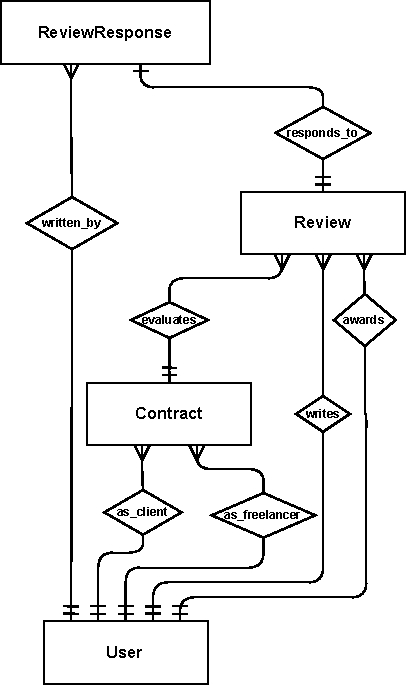
\includegraphics[width=0.52\textwidth]{image/ERD/ERD-ERD17.drawio.pdf}
    \caption{Reviews \& Reputation ERD}
    \label{fig:erd-reviews--reputation}
\end{figure}

\Needspace{8\baselineskip}
\paragraph*{b) Table of entities}\nopagebreak[4]
\begin{center}\nopagebreak[4]
\small\sloppy
\begin{longtable}{|L{2.5cm}|L{9.5cm}|}
\hline
\rowcolor{fptHeader}\textbf{Entity} & \textbf{Fields and descriptions} \\* \hline
\endfirsthead
\hline
\rowcolor{fptHeader}\textbf{Entity} & \textbf{Fields and descriptions} \\* \hline
\endhead
\hline\endfoot
\endlastfoot
\texttt{Contract} & - id: used to store the unique identifier of the record \\*
& - slug: used to store the URL slug \\
& - job\allowbreak Id: used to store the foreign key reference to the job \\
& - proposal\allowbreak Id: used to store the foreign key reference to the proposal \\
& - client\allowbreak Id: used to store the foreign key reference to the client \\
& - freelancer\allowbreak Id: used to store the foreign key reference to the freelancer \\
& - terms: used to store the contract terms text \\
& - total\allowbreak Amount: used to store the total amount \\
& - status: used to store the status value from the ContractStatus enumeration \\
& - signed\allowbreak By\allowbreak Client: used to store whether the contract is signed by the client \\
& - signed\allowbreak By\allowbreak Freelancer: used to store whether the contract is signed by the freelancer \\
& - client\allowbreak Signed\allowbreak At: used to store the client signing timestamp \\
& - freelancer\allowbreak Signed\allowbreak At: used to store the freelancer signing timestamp \\
& - client\allowbreak Platform\allowbreak Fee: used to store the client platform fee amount \\
& - platform\allowbreak Fee: used to store the platform fee amount \\
& - platform\allowbreak Fee\allowbreak Status: used to store the platform fee status value from the PlatformFeeStatus enumeration \\
& - platform\allowbreak Fee\allowbreak Paid\allowbreak At: used to store the platform fee payment timestamp \\
& - client\allowbreak Fee\allowbreak Status: used to store the client fee status value from the PlatformFeeStatus enumeration \\
& - client\allowbreak Fee\allowbreak Paid\allowbreak At: used to store the client fee payment timestamp \\
& - freelancer\allowbreak Fee\allowbreak Status: used to store the freelancer fee status value from the PlatformFeeStatus enumeration \\
& - freelancer\allowbreak Fee\allowbreak Paid\allowbreak At: used to store the freelancer fee payment timestamp \\
& - hold\allowbreak Payment\allowbreak Intent\allowbreak Id: used to store the hold payment intent id text value \\
& - hold\allowbreak Milestone\allowbreak Ids: used to store the list of hold milestone ids \\
& - rejected\allowbreak At: used to store the rejection timestamp \\
& - reject\allowbreak Reason: used to store the rejection reason text \\
& - created\allowbreak At: used to store the creation timestamp \\
& - signed\allowbreak At: used to store the signing timestamp \\
& - completed\allowbreak At: used to store the completion timestamp \\
& - expires\allowbreak At: used to store the expiration timestamp \\
& - deleted\allowbreak At: used to store the soft-deletion timestamp \\ \hline
\texttt{User} & - id: used to store the unique identifier of the record \\*
& - email: used to store the account email address \\
& - password: used to store the hashed account password \\
& - is\allowbreak Banned: used to store whether the account is banned \\
& - created\allowbreak At: used to store the creation timestamp \\
& - updated\allowbreak At: used to store the last update timestamp \\
& - deleted\allowbreak At: used to store the soft-deletion timestamp \\
& - stripe\allowbreak Customer\allowbreak Id: used to store the stripe customer id text value \\
& - stripe\allowbreak Account\allowbreak Id: used to store the stripe account id text value \\
& - stripe\allowbreak Onboarding\allowbreak Completed: used to store whether Stripe onboarding is completed \\
& - role\allowbreak Id: used to store the foreign key reference to the primary role \\ \hline
\texttt{Review} & - id: used to store the unique identifier of the record \\*
& - contract\allowbreak Id: used to store the foreign key reference to the contract \\
& - reviewer\allowbreak Id: used to store the foreign key reference to the reviewer \\
& - reviewee\allowbreak Id: used to store the foreign key reference to the reviewee \\
& - overall\allowbreak Rating: used to store the overall rating \\
& - breakdown: used to store the rating breakdown in JSON format \\
& - comment: used to store the comment text \\
& - created\allowbreak At: used to store the creation timestamp \\
& - updated\allowbreak At: used to store the last update timestamp \\
& - deleted\allowbreak At: used to store the soft-deletion timestamp \\ \hline
\texttt{Review\allowbreak Response} & - id: used to store the unique identifier of the record \\*
& - review\allowbreak Id: used to store the foreign key reference to the review \\
& - user\allowbreak Id: used to store the foreign key reference to the user \\
& - response\allowbreak Text: used to store the response text \\
& - created\allowbreak At: used to store the creation timestamp \\
& - updated\allowbreak At: used to store the last update timestamp \\
& - deleted\allowbreak At: used to store the soft-deletion timestamp \\ \hline
\end{longtable}
\end{center}

% ===============================================
% 4.1.5.19 ERD18
% ===============================================
\Needspace{12\baselineskip}
\paragraph{Forum Posts \& Comments}

This ERD describes the Forum Posts \& Comments module. It stores forum categories, posts, and comments. These tables support forum discussions and moderation.

\Needspace{12\baselineskip}
\paragraph*{a) ERD}
\begin{figure}[H]
    \centering
    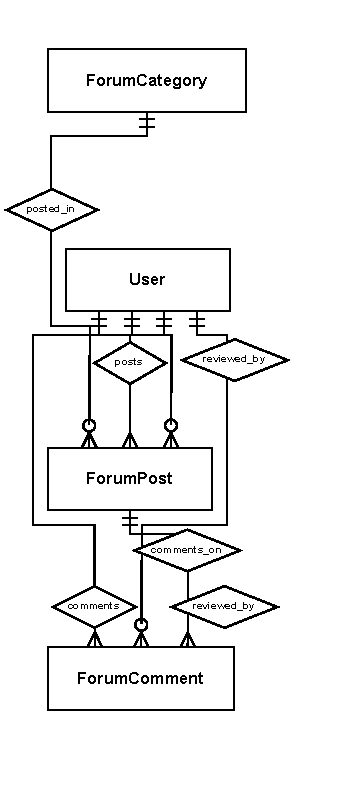
\includegraphics[width=0.78\textwidth]{image/ERD/ERD-ERD18.drawio.pdf}
    \caption{Forum Posts \& Comments ERD}
    \label{fig:erd-forum-posts--comments}
\end{figure}

\Needspace{8\baselineskip}
\paragraph*{b) Table of entities}\nopagebreak[4]
\begin{center}\nopagebreak[4]
\small\sloppy
\begin{longtable}{|L{2.5cm}|L{9.5cm}|}
\hline
\rowcolor{fptHeader}\textbf{Entity} & \textbf{Fields and descriptions} \\* \hline
\endfirsthead
\hline
\rowcolor{fptHeader}\textbf{Entity} & \textbf{Fields and descriptions} \\* \hline
\endhead
\hline\endfoot
\endlastfoot
\texttt{Forum\allowbreak Category} & - id: used to store the unique identifier of the record \\*
& - name: used to store the name value \\
& - slug: used to store the URL slug \\
& - description: used to store the description text \\
& - created\allowbreak At: used to store the creation timestamp \\
& - updated\allowbreak At: used to store the last update timestamp \\
& - deleted\allowbreak At: used to store the soft-deletion timestamp \\ \hline
\texttt{Forum\allowbreak Post} & - id: used to store the unique identifier of the record \\*
& - category\allowbreak Id: used to store the foreign key reference to the forum category \\
& - user\allowbreak Id: used to store the foreign key reference to the user \\
& - title: used to store the title text \\
& - slug: used to store the URL slug \\
& - content: used to store the content text \\
& - moderation\allowbreak Status: used to store the moderation status value from the ForumPostStatus enumeration \\
& - moderation\allowbreak Score: used to store the moderation score \\
& - moderation\allowbreak Categories: used to store the moderation categories in JSON format \\
& - moderation\allowbreak Message: used to store the moderation message text value \\
& - moderation\allowbreak Language: used to store the moderation language text value \\
& - reviewed\allowbreak By\allowbreak Id: used to store the foreign key reference to the reviewing administrator \\
& - reviewed\allowbreak At: used to store the review timestamp \\
& - created\allowbreak At: used to store the creation timestamp \\
& - updated\allowbreak At: used to store the last update timestamp \\
& - deleted\allowbreak At: used to store the soft-deletion timestamp \\ \hline
\texttt{User} & - id: used to store the unique identifier of the record \\*
& - email: used to store the account email address \\
& - password: used to store the hashed account password \\
& - is\allowbreak Banned: used to store whether the account is banned \\
& - created\allowbreak At: used to store the creation timestamp \\
& - updated\allowbreak At: used to store the last update timestamp \\
& - deleted\allowbreak At: used to store the soft-deletion timestamp \\
& - stripe\allowbreak Customer\allowbreak Id: used to store the stripe customer id text value \\
& - stripe\allowbreak Account\allowbreak Id: used to store the stripe account id text value \\
& - stripe\allowbreak Onboarding\allowbreak Completed: used to store whether Stripe onboarding is completed \\
& - role\allowbreak Id: used to store the foreign key reference to the primary role \\ \hline
\texttt{Forum\allowbreak Comment} & - id: used to store the unique identifier of the record \\*
& - post\allowbreak Id: used to store the foreign key reference to the forum post \\
& - user\allowbreak Id: used to store the foreign key reference to the user \\
& - content: used to store the content text \\
& - moderation\allowbreak Status: used to store the moderation status value from the ForumPostStatus enumeration \\
& - moderation\allowbreak Score: used to store the moderation score \\
& - moderation\allowbreak Categories: used to store the moderation categories in JSON format \\
& - moderation\allowbreak Message: used to store the moderation message text value \\
& - moderation\allowbreak Language: used to store the moderation language text value \\
& - reviewed\allowbreak By\allowbreak Id: used to store the foreign key reference to the reviewing administrator \\
& - reviewed\allowbreak At: used to store the review timestamp \\
& - created\allowbreak At: used to store the creation timestamp \\
& - updated\allowbreak At: used to store the last update timestamp \\
& - deleted\allowbreak At: used to store the soft-deletion timestamp \\ \hline
\end{longtable}
\end{center}

% ===============================================
% 4.1.5.20 ERD19
% ===============================================
\Needspace{12\baselineskip}
\paragraph{Forum Likes}

This ERD describes the Forum Likes module. It stores likes on posts and comments. These tables support reactions.

\Needspace{12\baselineskip}
\paragraph*{a) ERD}
\begin{figure}[H]
    \centering
    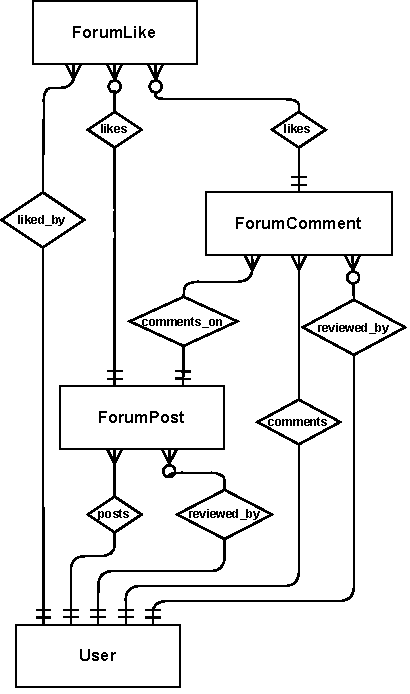
\includegraphics[width=0.52\textwidth]{image/ERD/ERD-ERD19.drawio.pdf}
    \caption{Forum Likes ERD}
    \label{fig:erd-forum-likes}
\end{figure}

\Needspace{8\baselineskip}
\paragraph*{b) Table of entities}\nopagebreak[4]
\begin{center}\nopagebreak[4]
\small\sloppy
\begin{longtable}{|L{2.5cm}|L{9.5cm}|}
\hline
\rowcolor{fptHeader}\textbf{Entity} & \textbf{Fields and descriptions} \\* \hline
\endfirsthead
\hline
\rowcolor{fptHeader}\textbf{Entity} & \textbf{Fields and descriptions} \\* \hline
\endhead
\hline\endfoot
\endlastfoot
\texttt{User} & - id: used to store the unique identifier of the record \\*
& - email: used to store the account email address \\
& - password: used to store the hashed account password \\
& - is\allowbreak Banned: used to store whether the account is banned \\
& - created\allowbreak At: used to store the creation timestamp \\
& - updated\allowbreak At: used to store the last update timestamp \\
& - deleted\allowbreak At: used to store the soft-deletion timestamp \\
& - stripe\allowbreak Customer\allowbreak Id: used to store the stripe customer id text value \\
& - stripe\allowbreak Account\allowbreak Id: used to store the stripe account id text value \\
& - stripe\allowbreak Onboarding\allowbreak Completed: used to store whether Stripe onboarding is completed \\
& - role\allowbreak Id: used to store the foreign key reference to the primary role \\ \hline
\texttt{Forum\allowbreak Post} & - id: used to store the unique identifier of the record \\*
& - category\allowbreak Id: used to store the foreign key reference to the forum category \\
& - user\allowbreak Id: used to store the foreign key reference to the user \\
& - title: used to store the title text \\
& - slug: used to store the URL slug \\
& - content: used to store the content text \\
& - moderation\allowbreak Status: used to store the moderation status value from the ForumPostStatus enumeration \\
& - moderation\allowbreak Score: used to store the moderation score \\
& - moderation\allowbreak Categories: used to store the moderation categories in JSON format \\
& - moderation\allowbreak Message: used to store the moderation message text value \\
& - moderation\allowbreak Language: used to store the moderation language text value \\
& - reviewed\allowbreak By\allowbreak Id: used to store the foreign key reference to the reviewing administrator \\
& - reviewed\allowbreak At: used to store the review timestamp \\
& - created\allowbreak At: used to store the creation timestamp \\
& - updated\allowbreak At: used to store the last update timestamp \\
& - deleted\allowbreak At: used to store the soft-deletion timestamp \\ \hline
\texttt{Forum\allowbreak Comment} & - id: used to store the unique identifier of the record \\*
& - post\allowbreak Id: used to store the foreign key reference to the forum post \\
& - user\allowbreak Id: used to store the foreign key reference to the user \\
& - content: used to store the content text \\
& - moderation\allowbreak Status: used to store the moderation status value from the ForumPostStatus enumeration \\
& - moderation\allowbreak Score: used to store the moderation score \\
& - moderation\allowbreak Categories: used to store the moderation categories in JSON format \\
& - moderation\allowbreak Message: used to store the moderation message text value \\
& - moderation\allowbreak Language: used to store the moderation language text value \\
& - reviewed\allowbreak By\allowbreak Id: used to store the foreign key reference to the reviewing administrator \\
& - reviewed\allowbreak At: used to store the review timestamp \\
& - created\allowbreak At: used to store the creation timestamp \\
& - updated\allowbreak At: used to store the last update timestamp \\
& - deleted\allowbreak At: used to store the soft-deletion timestamp \\ \hline
\texttt{Forum\allowbreak Like} & - id: used to store the unique identifier of the record \\*
& - user\allowbreak Id: used to store the foreign key reference to the user \\
& - post\allowbreak Id: used to store the foreign key reference to the forum post \\
& - comment\allowbreak Id: used to store the foreign key reference to the forum comment \\
& - reaction\allowbreak Type: used to store the reaction type text value \\
& - created\allowbreak At: used to store the creation timestamp \\ \hline
\end{longtable}
\end{center}

% ===============================================
% 4.1.5.21 ERD20
% ===============================================
\Needspace{12\baselineskip}
\paragraph{Forum Reports \& Moderation}

This ERD describes the Forum Reports \& Moderation module. It stores forum reports, moderation queue, and banned keywords. These tables support reporting content and admin moderation.

\Needspace{12\baselineskip}
\paragraph*{a) ERD}
\begin{figure}[H]
    \centering
    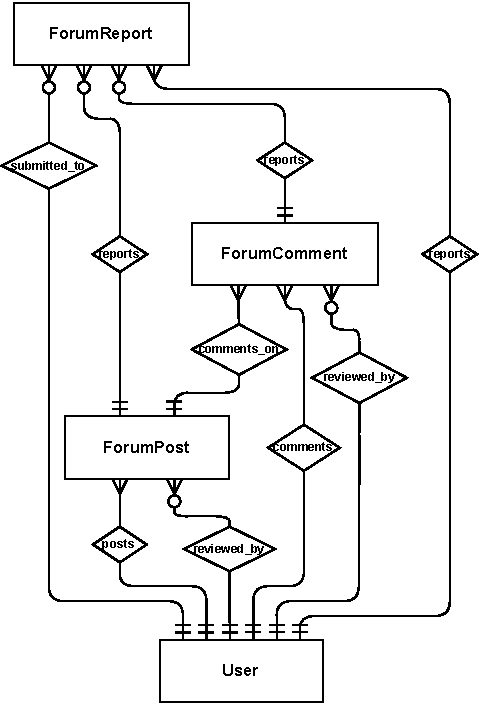
\includegraphics[width=0.52\textwidth]{image/ERD/ERD-ERD20.drawio.pdf}
    \caption{Forum Reports \& Moderation ERD}
    \label{fig:erd-forum-reports--moderation}
\end{figure}

\Needspace{8\baselineskip}
\paragraph*{b) Table of entities}\nopagebreak[4]
\begin{center}\nopagebreak[4]
\small\sloppy
\begin{longtable}{|L{2.5cm}|L{9.5cm}|}
\hline
\rowcolor{fptHeader}\textbf{Entity} & \textbf{Fields and descriptions} \\* \hline
\endfirsthead
\hline
\rowcolor{fptHeader}\textbf{Entity} & \textbf{Fields and descriptions} \\* \hline
\endhead
\hline\endfoot
\endlastfoot
\texttt{User} & - id: used to store the unique identifier of the record \\*
& - email: used to store the account email address \\
& - password: used to store the hashed account password \\
& - is\allowbreak Banned: used to store whether the account is banned \\
& - created\allowbreak At: used to store the creation timestamp \\
& - updated\allowbreak At: used to store the last update timestamp \\
& - deleted\allowbreak At: used to store the soft-deletion timestamp \\
& - stripe\allowbreak Customer\allowbreak Id: used to store the stripe customer id text value \\
& - stripe\allowbreak Account\allowbreak Id: used to store the stripe account id text value \\
& - stripe\allowbreak Onboarding\allowbreak Completed: used to store whether Stripe onboarding is completed \\
& - role\allowbreak Id: used to store the foreign key reference to the primary role \\ \hline
\texttt{Forum\allowbreak Post} & - id: used to store the unique identifier of the record \\*
& - category\allowbreak Id: used to store the foreign key reference to the forum category \\
& - user\allowbreak Id: used to store the foreign key reference to the user \\
& - title: used to store the title text \\
& - slug: used to store the URL slug \\
& - content: used to store the content text \\
& - moderation\allowbreak Status: used to store the moderation status value from the ForumPostStatus enumeration \\
& - moderation\allowbreak Score: used to store the moderation score \\
& - moderation\allowbreak Categories: used to store the moderation categories in JSON format \\
& - moderation\allowbreak Message: used to store the moderation message text value \\
& - moderation\allowbreak Language: used to store the moderation language text value \\
& - reviewed\allowbreak By\allowbreak Id: used to store the foreign key reference to the reviewing administrator \\
& - reviewed\allowbreak At: used to store the review timestamp \\
& - created\allowbreak At: used to store the creation timestamp \\
& - updated\allowbreak At: used to store the last update timestamp \\
& - deleted\allowbreak At: used to store the soft-deletion timestamp \\ \hline
\texttt{Forum\allowbreak Comment} & - id: used to store the unique identifier of the record \\*
& - post\allowbreak Id: used to store the foreign key reference to the forum post \\
& - user\allowbreak Id: used to store the foreign key reference to the user \\
& - content: used to store the content text \\
& - moderation\allowbreak Status: used to store the moderation status value from the ForumPostStatus enumeration \\
& - moderation\allowbreak Score: used to store the moderation score \\
& - moderation\allowbreak Categories: used to store the moderation categories in JSON format \\
& - moderation\allowbreak Message: used to store the moderation message text value \\
& - moderation\allowbreak Language: used to store the moderation language text value \\
& - reviewed\allowbreak By\allowbreak Id: used to store the foreign key reference to the reviewing administrator \\
& - reviewed\allowbreak At: used to store the review timestamp \\
& - created\allowbreak At: used to store the creation timestamp \\
& - updated\allowbreak At: used to store the last update timestamp \\
& - deleted\allowbreak At: used to store the soft-deletion timestamp \\ \hline
\texttt{Forum\allowbreak Report} & - id: used to store the unique identifier of the record \\*
& - reporter\allowbreak Id: used to store the foreign key reference to the reporting user \\
& - post\allowbreak Id: used to store the foreign key reference to the forum post \\
& - comment\allowbreak Id: used to store the foreign key reference to the forum comment \\
& - reason: used to store the reason text \\
& - status: used to store the status value from the ReportStatus enumeration \\
& - admin\allowbreak Id: used to store the foreign key reference to the reviewing administrator \\
& - created\allowbreak At: used to store the creation timestamp \\ \hline
\end{longtable}
\end{center}

% ===============================================
% 4.1.5.22 ERD21
% ===============================================
\Needspace{12\baselineskip}
\paragraph{Messaging \& Notifications}

This ERD describes the Messaging \& Notifications module. It stores notifications, conversations, and direct messages. These tables support real-time chat and in-app notifications.

\Needspace{12\baselineskip}
\paragraph*{a) ERD}
\begin{figure}[H]
    \centering
    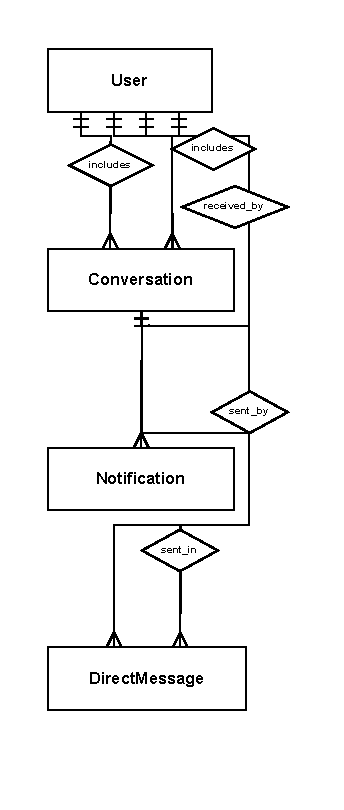
\includegraphics[width=0.78\textwidth]{image/ERD/ERD-ERD21.drawio.pdf}
    \caption{Messaging \& Notifications ERD}
    \label{fig:erd-messaging--notifications}
\end{figure}

\Needspace{8\baselineskip}
\paragraph*{b) Table of entities}\nopagebreak[4]
\begin{center}\nopagebreak[4]
\small\sloppy
\begin{longtable}{|L{2.5cm}|L{9.5cm}|}
\hline
\rowcolor{fptHeader}\textbf{Entity} & \textbf{Fields and descriptions} \\* \hline
\endfirsthead
\hline
\rowcolor{fptHeader}\textbf{Entity} & \textbf{Fields and descriptions} \\* \hline
\endhead
\hline\endfoot
\endlastfoot
\texttt{User} & - id: used to store the unique identifier of the record \\*
& - email: used to store the account email address \\
& - password: used to store the hashed account password \\
& - is\allowbreak Banned: used to store whether the account is banned \\
& - created\allowbreak At: used to store the creation timestamp \\
& - updated\allowbreak At: used to store the last update timestamp \\
& - deleted\allowbreak At: used to store the soft-deletion timestamp \\
& - stripe\allowbreak Customer\allowbreak Id: used to store the stripe customer id text value \\
& - stripe\allowbreak Account\allowbreak Id: used to store the stripe account id text value \\
& - stripe\allowbreak Onboarding\allowbreak Completed: used to store whether Stripe onboarding is completed \\
& - role\allowbreak Id: used to store the foreign key reference to the primary role \\ \hline
\texttt{Conversation} & - id: used to store the unique identifier of the record \\*
& - slug: used to store the URL slug \\
& - participant1: used to store the foreign key reference to the first participant \\
& - participant2: used to store the foreign key reference to the second participant \\
& - created\allowbreak At: used to store the creation timestamp \\
& - deleted\allowbreak At: used to store the soft-deletion timestamp \\
& - participant1\allowbreak Hidden\allowbreak At: used to store the participant1 hidden at timestamp \\
& - participant2\allowbreak Hidden\allowbreak At: used to store the participant2 hidden at timestamp \\
& - participant1\allowbreak Pinned\allowbreak At: used to store the participant1 pinned at timestamp \\
& - participant2\allowbreak Pinned\allowbreak At: used to store the participant2 pinned at timestamp \\ \hline
\texttt{Direct\allowbreak Message} & - id: used to store the unique identifier of the record \\*
& - conversation\allowbreak Id: used to store the foreign key reference to the conversation \\
& - sender\allowbreak Id: used to store the foreign key reference to the sending user \\
& - message: used to store the message text \\
& - file\allowbreak Url: used to store the file URL \\
& - file\allowbreak Name: used to store the uploaded file name \\
& - file\allowbreak Size: used to store the file size in bytes \\
& - file\allowbreak Type: used to store the file type text value \\
& - is\allowbreak Read: used to store whether the record is read \\
& - created\allowbreak At: used to store the creation timestamp \\
& - deleted\allowbreak At: used to store the soft-deletion timestamp \\ \hline
\texttt{Notification} & - id: used to store the unique identifier of the record \\*
& - user\allowbreak Id: used to store the foreign key reference to the user \\
& - type: used to store the type value from the NotificationType enumeration \\
& - title: used to store the title text \\
& - message: used to store the message text \\
& - data: used to store the data data in JSON format \\
& - is\allowbreak Read: used to store whether the record is read \\
& - created\allowbreak At: used to store the creation timestamp \\
& - deleted\allowbreak At: used to store the soft-deletion timestamp \\ \hline
\end{longtable}
\end{center}

% ===============================================
% 4.1.5.23 ERD22
% ===============================================
\Needspace{12\baselineskip}
\paragraph{Administration \& System}

This ERD describes the Administration \& System module. It stores announcement banners, system settings, and advertisement banners. These tables support admin configuration and banners.

\Needspace{12\baselineskip}
\paragraph*{a) ERD}
\begin{figure}[H]
    \centering
    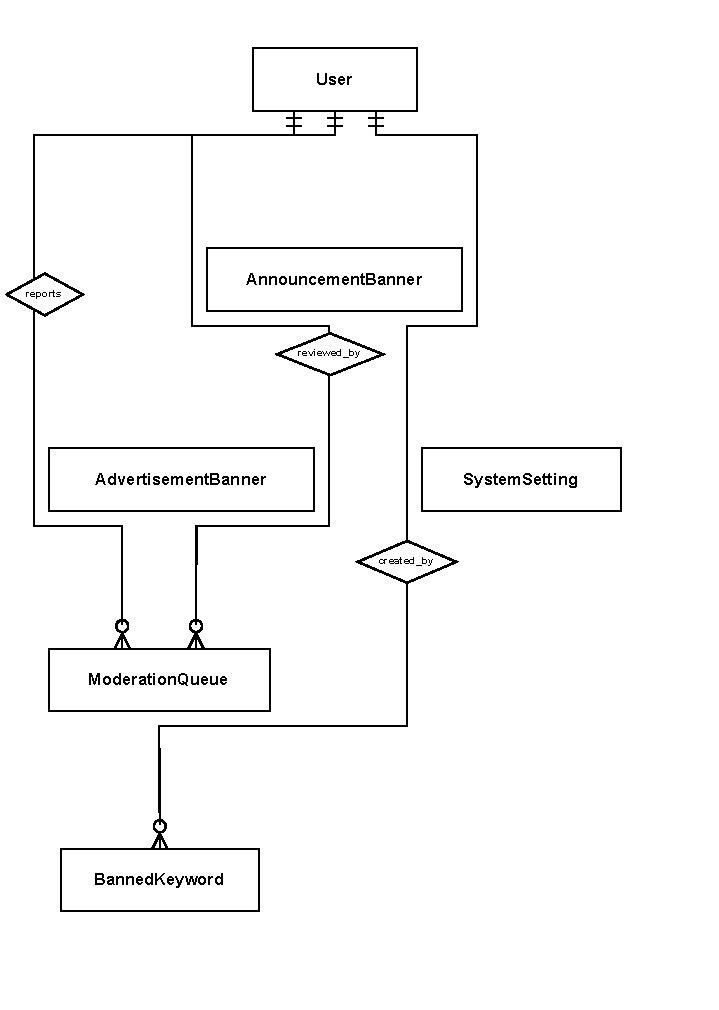
\includegraphics[width=0.78\textwidth]{image/ERD/ERD-ERD22.drawio.pdf}
    \caption{Administration \& System ERD}
    \label{fig:erd-administration--system}
\end{figure}

\Needspace{8\baselineskip}
\paragraph*{b) Table of entities}\nopagebreak[4]
\begin{center}\nopagebreak[4]
\small\sloppy
\begin{longtable}{|L{2.5cm}|L{9.5cm}|}
\hline
\rowcolor{fptHeader}\textbf{Entity} & \textbf{Fields and descriptions} \\* \hline
\endfirsthead
\hline
\rowcolor{fptHeader}\textbf{Entity} & \textbf{Fields and descriptions} \\* \hline
\endhead
\hline\endfoot
\endlastfoot
\texttt{User} & - id: used to store the unique identifier of the record \\*
& - email: used to store the account email address \\
& - password: used to store the hashed account password \\
& - is\allowbreak Banned: used to store whether the account is banned \\
& - created\allowbreak At: used to store the creation timestamp \\
& - updated\allowbreak At: used to store the last update timestamp \\
& - deleted\allowbreak At: used to store the soft-deletion timestamp \\
& - stripe\allowbreak Customer\allowbreak Id: used to store the stripe customer id text value \\
& - stripe\allowbreak Account\allowbreak Id: used to store the stripe account id text value \\
& - stripe\allowbreak Onboarding\allowbreak Completed: used to store whether Stripe onboarding is completed \\
& - role\allowbreak Id: used to store the foreign key reference to the primary role \\ \hline
\texttt{Moderation\allowbreak Queue} & - id: used to store the unique identifier of the record \\*
& - content\allowbreak Type: used to store the content type value from the ModerationContentType enumeration \\
& - content\allowbreak Id: used to store the content id integer value \\
& - reporter\allowbreak Id: used to store the foreign key reference to the reporting user \\
& - reason: used to store the reason text \\
& - status: used to store the status value from the ReportStatus enumeration \\
& - admin\allowbreak Id: used to store the foreign key reference to the reviewing administrator \\
& - action\allowbreak Taken: used to store the moderation action text \\
& - created\allowbreak At: used to store the creation timestamp \\
& - resolved\allowbreak At: used to store the resolution timestamp \\ \hline
\texttt{Banned\allowbreak Keyword} & - id: used to store the unique identifier of the record \\*
& - keyword: used to store the banned keyword text \\
& - created\allowbreak By: used to store the foreign key reference to the user \\
& - created\allowbreak At: used to store the creation timestamp \\ \hline
\texttt{Announcement\allowbreak Banner} & - id: used to store the unique identifier of the record \\*
& - message: used to store the message text \\
& - link: used to store the banner link \\
& - start\allowbreak Date: used to store the start date timestamp \\
& - end\allowbreak Date: used to store the end date timestamp \\
& - is\allowbreak Active: used to store whether the record is active \\
& - created\allowbreak At: used to store the creation timestamp \\
& - updated\allowbreak At: used to store the last update timestamp \\
& - deleted\allowbreak At: used to store the soft-deletion timestamp \\ \hline
\texttt{Advertisement\allowbreak Banner} & - id: used to store the unique identifier of the record \\*
& - title: used to store the title text \\
& - image\allowbreak Url: used to store the banner image URL \\
& - link\allowbreak Url: used to store the link URL \\
& - position: used to store the position value from the BannerPosition enumeration \\
& - start\allowbreak Date: used to store the start date timestamp \\
& - end\allowbreak Date: used to store the end date timestamp \\
& - is\allowbreak Active: used to store whether the record is active \\
& - created\allowbreak At: used to store the creation timestamp \\
& - updated\allowbreak At: used to store the last update timestamp \\ \hline
\texttt{System\allowbreak Setting} & - id: used to store the unique identifier of the record \\*
& - key: used to store the setting key \\
& - value: used to store the setting value \\
& - created\allowbreak At: used to store the creation timestamp \\
& - updated\allowbreak At: used to store the last update timestamp \\ \hline
\end{longtable}
\end{center}
